\vspace{-0.2cm}
\section{Experiments}
\vspace{-0.2cm}
We perform a suite of experiments on synthetic and real-world datasets to evaluate our attention based interpretable fairness framework. First, we elucidate %(demonstrate?)
interpretability on the synthetic dataset on which we can control the relations between input and output features. We verify that our interpretability framework recovers expected attributions and behaviour. We also demonstrate interpretability on the real-world dataset and identify features that cause unfairness.  Exploiting these attributions, we test our proposed post-processing bias mitigation framework and compare it with various recent mitigation approaches. Finally, we show the effectiveness of our mitigation approach on non-tabular data format, namely text.

\subsection{Datasets}

\newcommand{\bern}{\text{Ber}}

\subsubsection{Synthetic Data} \label{syn_data_sec}
% TODO: revisit this
To validate the interpretability framework, we created two synthetic datasets in which we control how features interact with each other and contribute to the accuracy and fairness of the outcome variable.
These datasets capture some of the common scenarios arising in decision or classification problems.
% phenomenons that occur in  and performed our first set of experiments.

\paragraph{Scenario 1:} First, we create a simple scenario to demonstrate that our framework identifies correct feature attributions for fairness and accuracy. To this end, we create a feature that is correlated with the outcome (responsible for accuracy), a discrete feature that would cause the prediction outcomes to be biased (responsible for fairness), and a continuous feature that is independent of the label or the task; thus, irrelevant for the task. Intuitively, suppose the attention-based interpretability framework works correctly. In that case, we expect to see a reduction in accuracy upon removing (i.e., making the attention weight zero) the feature responsible  for the accuracy, reduction in bias upon removing the feature responsible for bias, and very little or no change upon removing the irrelevant feature. With this objective, we generated a synthetic dataset with three features, i.e., $x = [f_1, f_2, f_3]$ as follows~\footnote{We use $x\sim \bern(p)$ to denote that $x$  is a Bernoulli random variable with $P(x=1)=p$.}.
\begin{equation*}
    f_1 ~\sim \bern(0.9)
    % \sim \begin{cases}
    %     \bern(0.9) & \text{if } y=1\\
    %     \bern(0.9) & \text{if } y=0
    % \end{cases}
    \quad f_2\sim \bern(0.5)
    \quad f_3\sim \mathcal N (0,1)
    \quad y\sim \begin{cases}
        \bern(0.9) & \text{if } f_2=1\\
        \bern(0.1) & \text{if } f_2=0
    \end{cases}
\end{equation*}
%
Clearly, $f_2$ has the most predictive information for the task and responsible for accuracy. Here, we consider $f_1$ as the sensitive attribute. $f_1$ is an imbalanced feature that can bias the outcome and is generated such that there is no intentional correlation between $f_1$ and the outcome, $y$ or $f_2$. $f_3$ is sampled from a normal distribution independent of the outcome $y$, or the other features, making it  irrelevant to the task.
Thus, an ideal classifier would be fair if it captures the correct outcome without being affected by the imbalance in $f_1$. However, due to limited data and skew in $f_1$,  there will be some undesired bias --- few errors when $f_1=0$ can lead to large statistical parity. 

 
% Due to the existing correlation between $f_2$ and the outcome variable $y$, $f_2$ can be considered as the feature with the most predictive information and responsible for accuracy. We consider $f_1$ as the sensitive attribute. It is generated such that there is no intentional correlation between $f_1$ and the outcome, $y$ or $f_2$. However, since $f_1$ is skewed towards $1$ and is the sensitive attribute over which statistical parity measure is applied, there will be some undesired bias. Lastly, we sample $f_3$ from normal distribution that it is independent of  the outcome $y$, or the other features; thus, making it  irrelevant to the task.

\paragraph{Scenario 2:} Using features that are not identified as sensitive attributes can result in unfair decisions due to their implicit relations or correlations with the sensitive attributes. This phenomenon is called indirect discrimination~\cite{zliobaite2015survey,6175897,ijcai2017-549}. We designed this synthetic dataset to demonstrate and characterize  the behavior of our framework under indirect discrimination. Similar to the previous scenario, we consider three features. Here,  $f_1$ is considered as the sensitive attribute, and $f_2$ is correlated with $f_1$ and the outcome, $y$. The generative process is as follows:
\begin{equation*}
    f_1\sim \begin{cases}
        \bern(0.9) & \text{if } f_2=1\\
        \bern(0.1) & \text{if } f_2=0
    \end{cases}
    \quad f_2\sim\bern(0.5)
    \quad f_3\sim \mathcal N (0,1)
    \quad y\sim \begin{cases}
        \bern(0.7) & \text{if } f_2=1\\
        \bern(0.3) & \text{if } f_2=0
    \end{cases}
\end{equation*}

Note that, in this case $f_1$ and $y$ are correlated with 
$f_2$. The model should mostly rely on $f_2$ for its decisions. 
However, due to the correlation between $f_1$ and $f_2$, we expect $f_2$ to affect both the accuracy and fairness of the model. Thus, in this case, indirect discrimination is possible. Using such a synthetic dataset, we demonstrate a) indirect discrimination and b) the need  to have  an interpretable framework to reason about unfairness and not blindly focus on the sensitive attributes for bias mitigation.


% Note that $f_1$ is made to be correlated with $f_2$, and similarly the outcome is made to be correlated with $f_2$. Thus, the model mostly will rely on $f_2$ for its decisions as $f_2$ is the feature that is making the outcome to be correlated with itself. Therefore, despite the fact that $f_1$ is the sensitive attribute, we expect $f_2$ to affect both accuracy and fairness of the model more than $f_1$ as it is directly correlated with both the outcome and $f_1$ showing how indirect discrimination is possible. Using such synthetic dataset, we demonstrate a) indirect discrimination, and b) the need for having an interpretable framework to reason about unfairness and not blindly focus on the sensitive attributes for bias mitigation.

\subsubsection{Real-world Datasets}
% we can also probably remove this introduction paragraph
In addition to synthetic datasets, we demonstrate our approach on various real-world datasets which we discuss next.
%  used the UCI Adult and Heritage Health datasets and observed how different features contribute to accuracy and fairness of the model in these real-world datasets.

\paragraph{Tabular Datasets:}
We conduct our experiments on two real-world tabular datasets often used to benchmark fair classification techniques --- \textit{UCI Adult}~\cite{Dua:2019} and \textit{Heritage Health}~\footnote{https://www.kaggle.com/c/hhp} datasets. The \textit{UCI Adult} dataset contains census information about individuals, with the prediction task being whether the income of the individual is higher than \$50k or not. The sensitive attribute, in this case, is gender (male/female).  The \textit{Heritage Health} dataset contains patient information, and the task is to predict the Charleson Index (comorbidity index, which is a patient survival indicator). Each patient is grouped into one of the 9 possible age groups, and we consider this as the sensitive attribute.  We used the same pre-processing and train-test splits as in~\cite{gupta2021controllable}.

\paragraph{Non-Tabular or Text Dataset:}
To demonstrate the flexibility of our approach, we also experiment with a non-tabular text dataset. We used the \textit{biosbias} dataset~\cite{de2019bias}. The dataset contains short bios of individuals. The task is to predict the occupation of the individual from their bio.
We utilized the bios from the year 2018 from the \texttt{2018\_34} archive and  considered two occupations for our experiments, namely, nurse and dentist. The dataset was split into $70-15-15$ train, validation, and test splits. \cite{de2019bias} has demonstrated the existence of gender bias in this prediction task and showed that certain gender words are associated with certain job types. For example, for the bios that we consider, we expect female associated words, such as \textit{she}, to cause skew towards the prediction of job nurse and male associated words, such as \textit{he}, to skew the prediction towards the job dentist.
% The goal of our study is to manipulate attention weights associated with the problematic features such as gender words, improve the performance of the model, and reduce the previously observed gender biases in this dataset.


% scenario, we wanted to observe the effect of the indirect discrimination, its extent, and whether it is possible for a non-sensitive attribute to play more important role on fairness of the model than the sensitive attribute itself. Thus, we specifically designed a scenario in which the non-sensitive attribute plays a more important role in creating unfairness than the sensitive attribute itself. This is done to show 1. the importance of indirect discrimination and 2. the need for having such interpretable framework to reason about unfairness and not blindly always put our focus on the sensitive attribute for bias mitigation. This data has three features same as the previous scenario, such that f1 is the sensitive attribute, f2 is sampled from Bernoulli distribution $f2 \mathtt{\sim} Bernoulli(0.5)$ and is correlated with both $f1$ and the outcome. Notice here $f1$ is made to be correlated with $f2$ and similarly the outcome is made to be correlated with $f2$. Thus, the model mostly will rely on $f2$ for its decisions as $f2$ is the feature that is making the outcome to be correlated with itself. Thus, despite the fact that $f1$ is the sensitive attribute, we expect $f2$ to affect both accuracy and fairness of the model more than $f1$ as it is both correlated with the outcome and $f1$ showing how indirect discrimination is possible.

% \begin{figure*}[t]
% \begin{subfigure}[b]{0.5\textwidth}
% 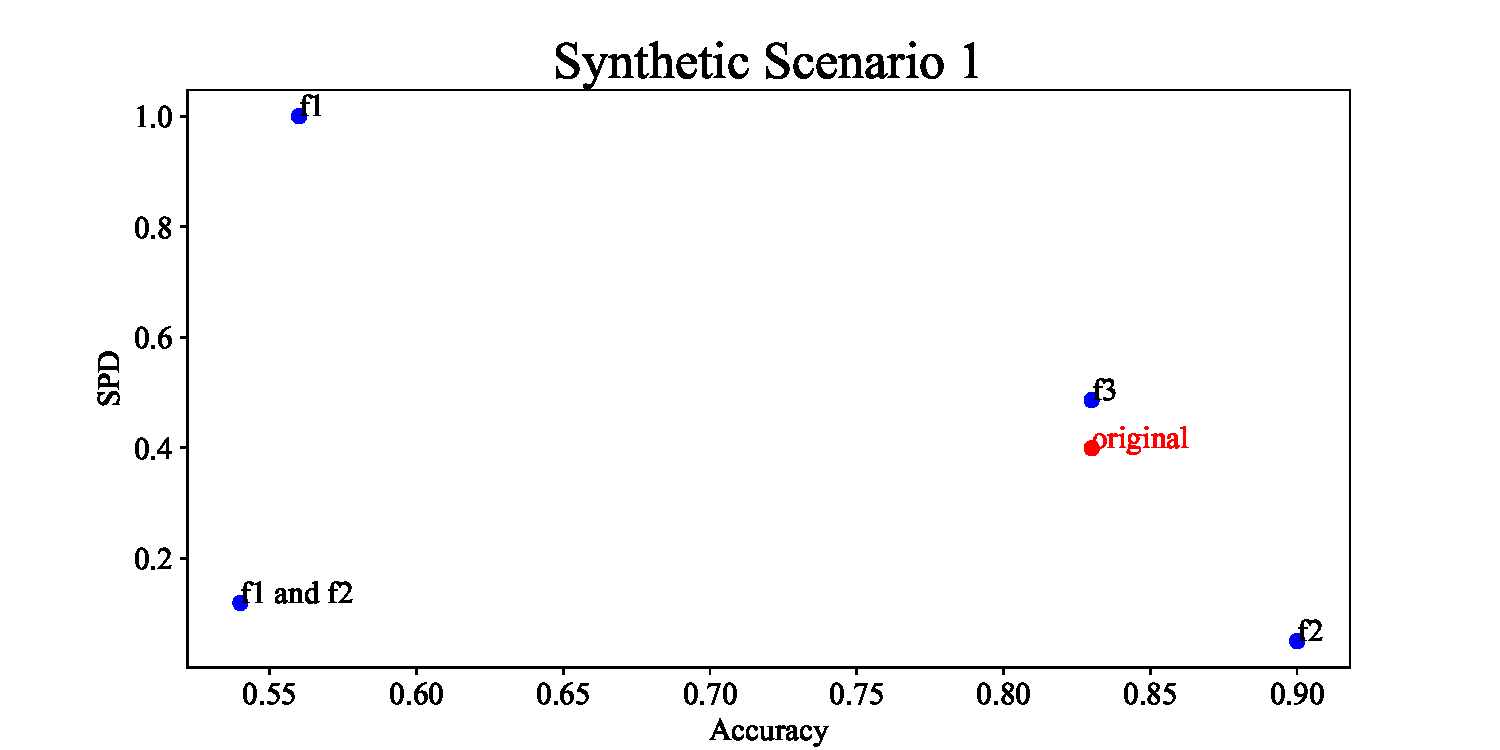
\includegraphics[width=\textwidth,trim=1cm 0cm 1.5cm 0cm,clip=true]{./images/inter_imgs/scen1.pdf}
% \end{subfigure}
% \begin{subfigure}[b]{0.5\textwidth}
% 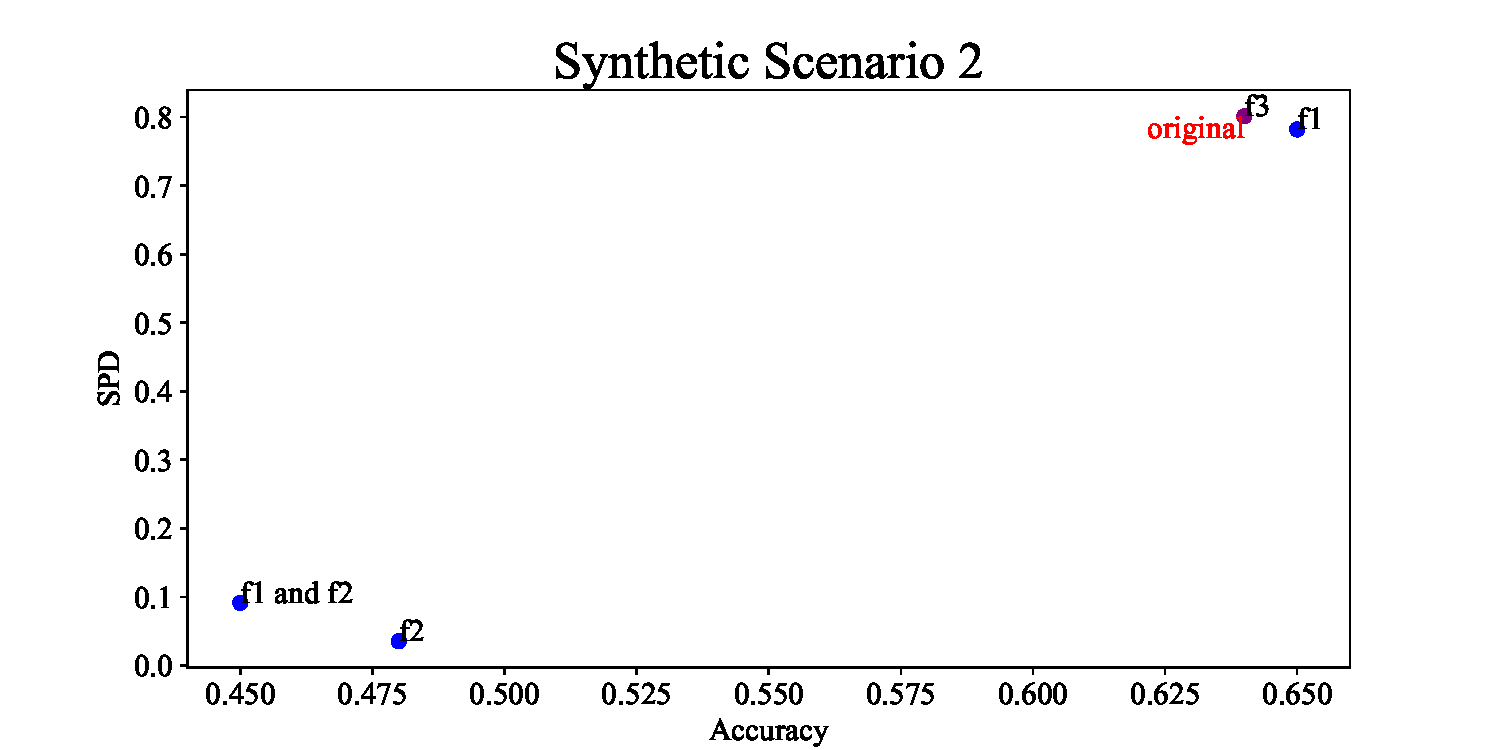
\includegraphics[width=\textwidth,trim=1cm 0cm 1.5cm 0cm,clip=true]{./images/inter_imgs/scen2.pdf}
% \end{subfigure}
% \begin{subfigure}[b]{0.5\textwidth}
% 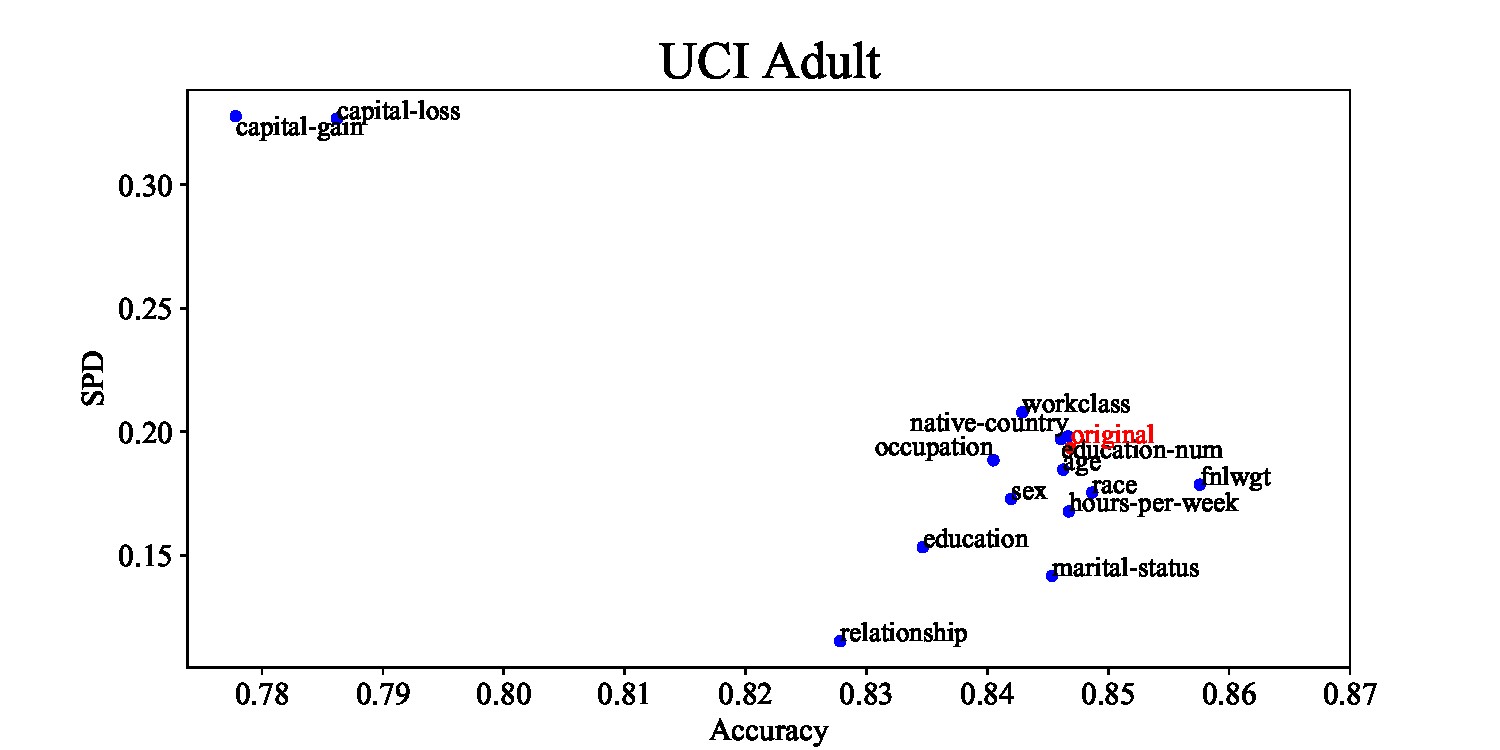
\includegraphics[width=\textwidth,trim=1cm 0cm 1.5cm 0cm,clip=true]{./images/inter_imgs/real_data_adult.pdf}
% \end{subfigure}
% \begin{subfigure}[b]{0.5\textwidth}
% 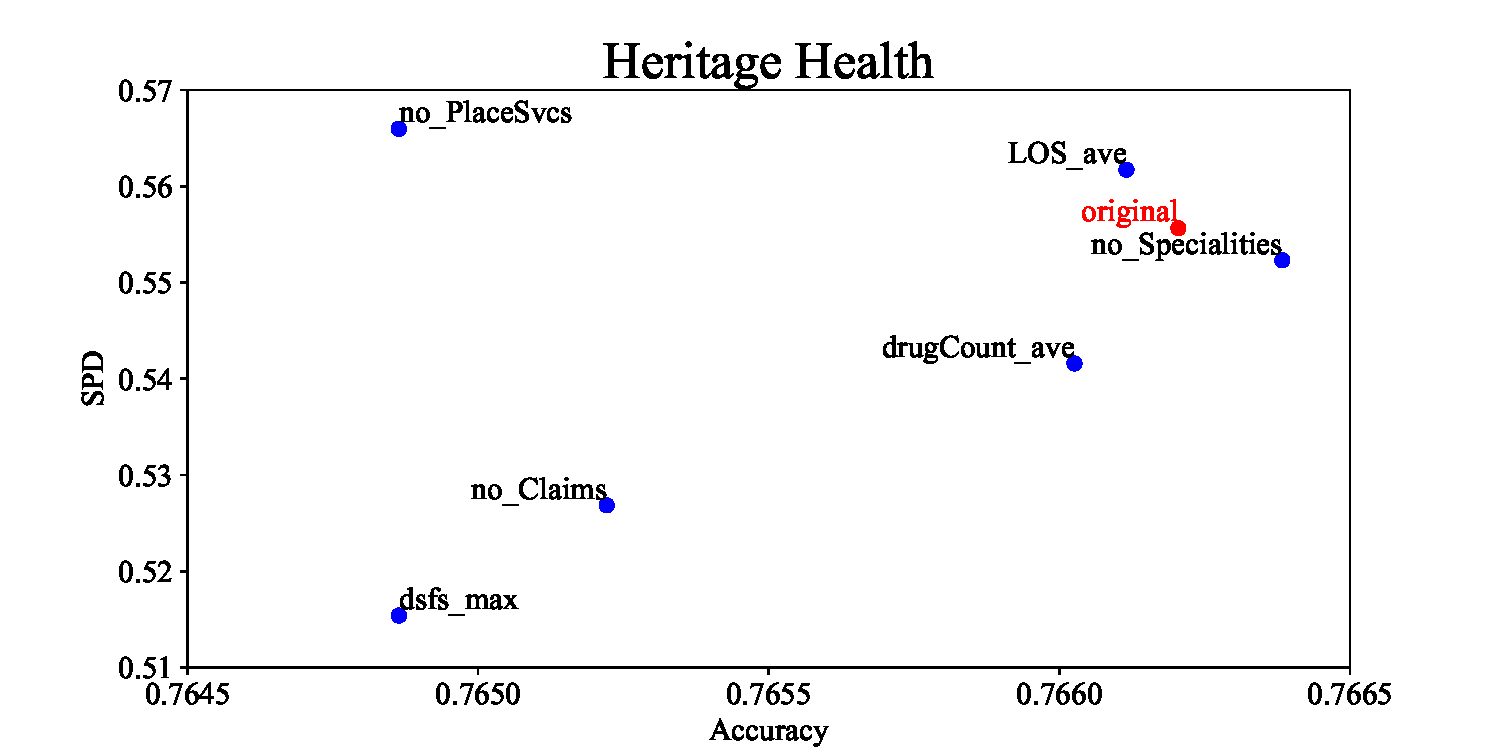
\includegraphics[width=\textwidth,trim=1cm 0cm 1.5cm 0cm,clip=true]{./images/inter_imgs/real_data_health_subset.pdf}
% \end{subfigure}
% \caption{Results from the synthetic datasets on top and real-world datasets in the bottom. Labels on the points represent the feature name that was removed. The results show how the accuracy and fairness of the model (in terms of statistical parity difference) change by exclusion of each feature. The red original point represents the results of the model including all the features.}
% \label{interpret_results}
% \end{figure*}




% \subsection{Attention and Fairness Interpretability}
% \subsection{Results}
\subsection{Interpreting Fairness with Attention}
\label{sec:interpret_fairness}
% Alternate Titles:
%  - Interpreting Fair Decisions
%  - Attributing Fairness
%  - Interpreting Fairness
% In this section, our plan is to show the effectiveness of our interpretability framework in being able to capture responsible features for each aspect of the model. To achiev  e this goal, we do some controlled experiments and show results on controlled synthetic setting as well as results on well-known real-wold datasets.
\begin{figure*}[t]
\begin{subfigure}[b]{0.5\textwidth}
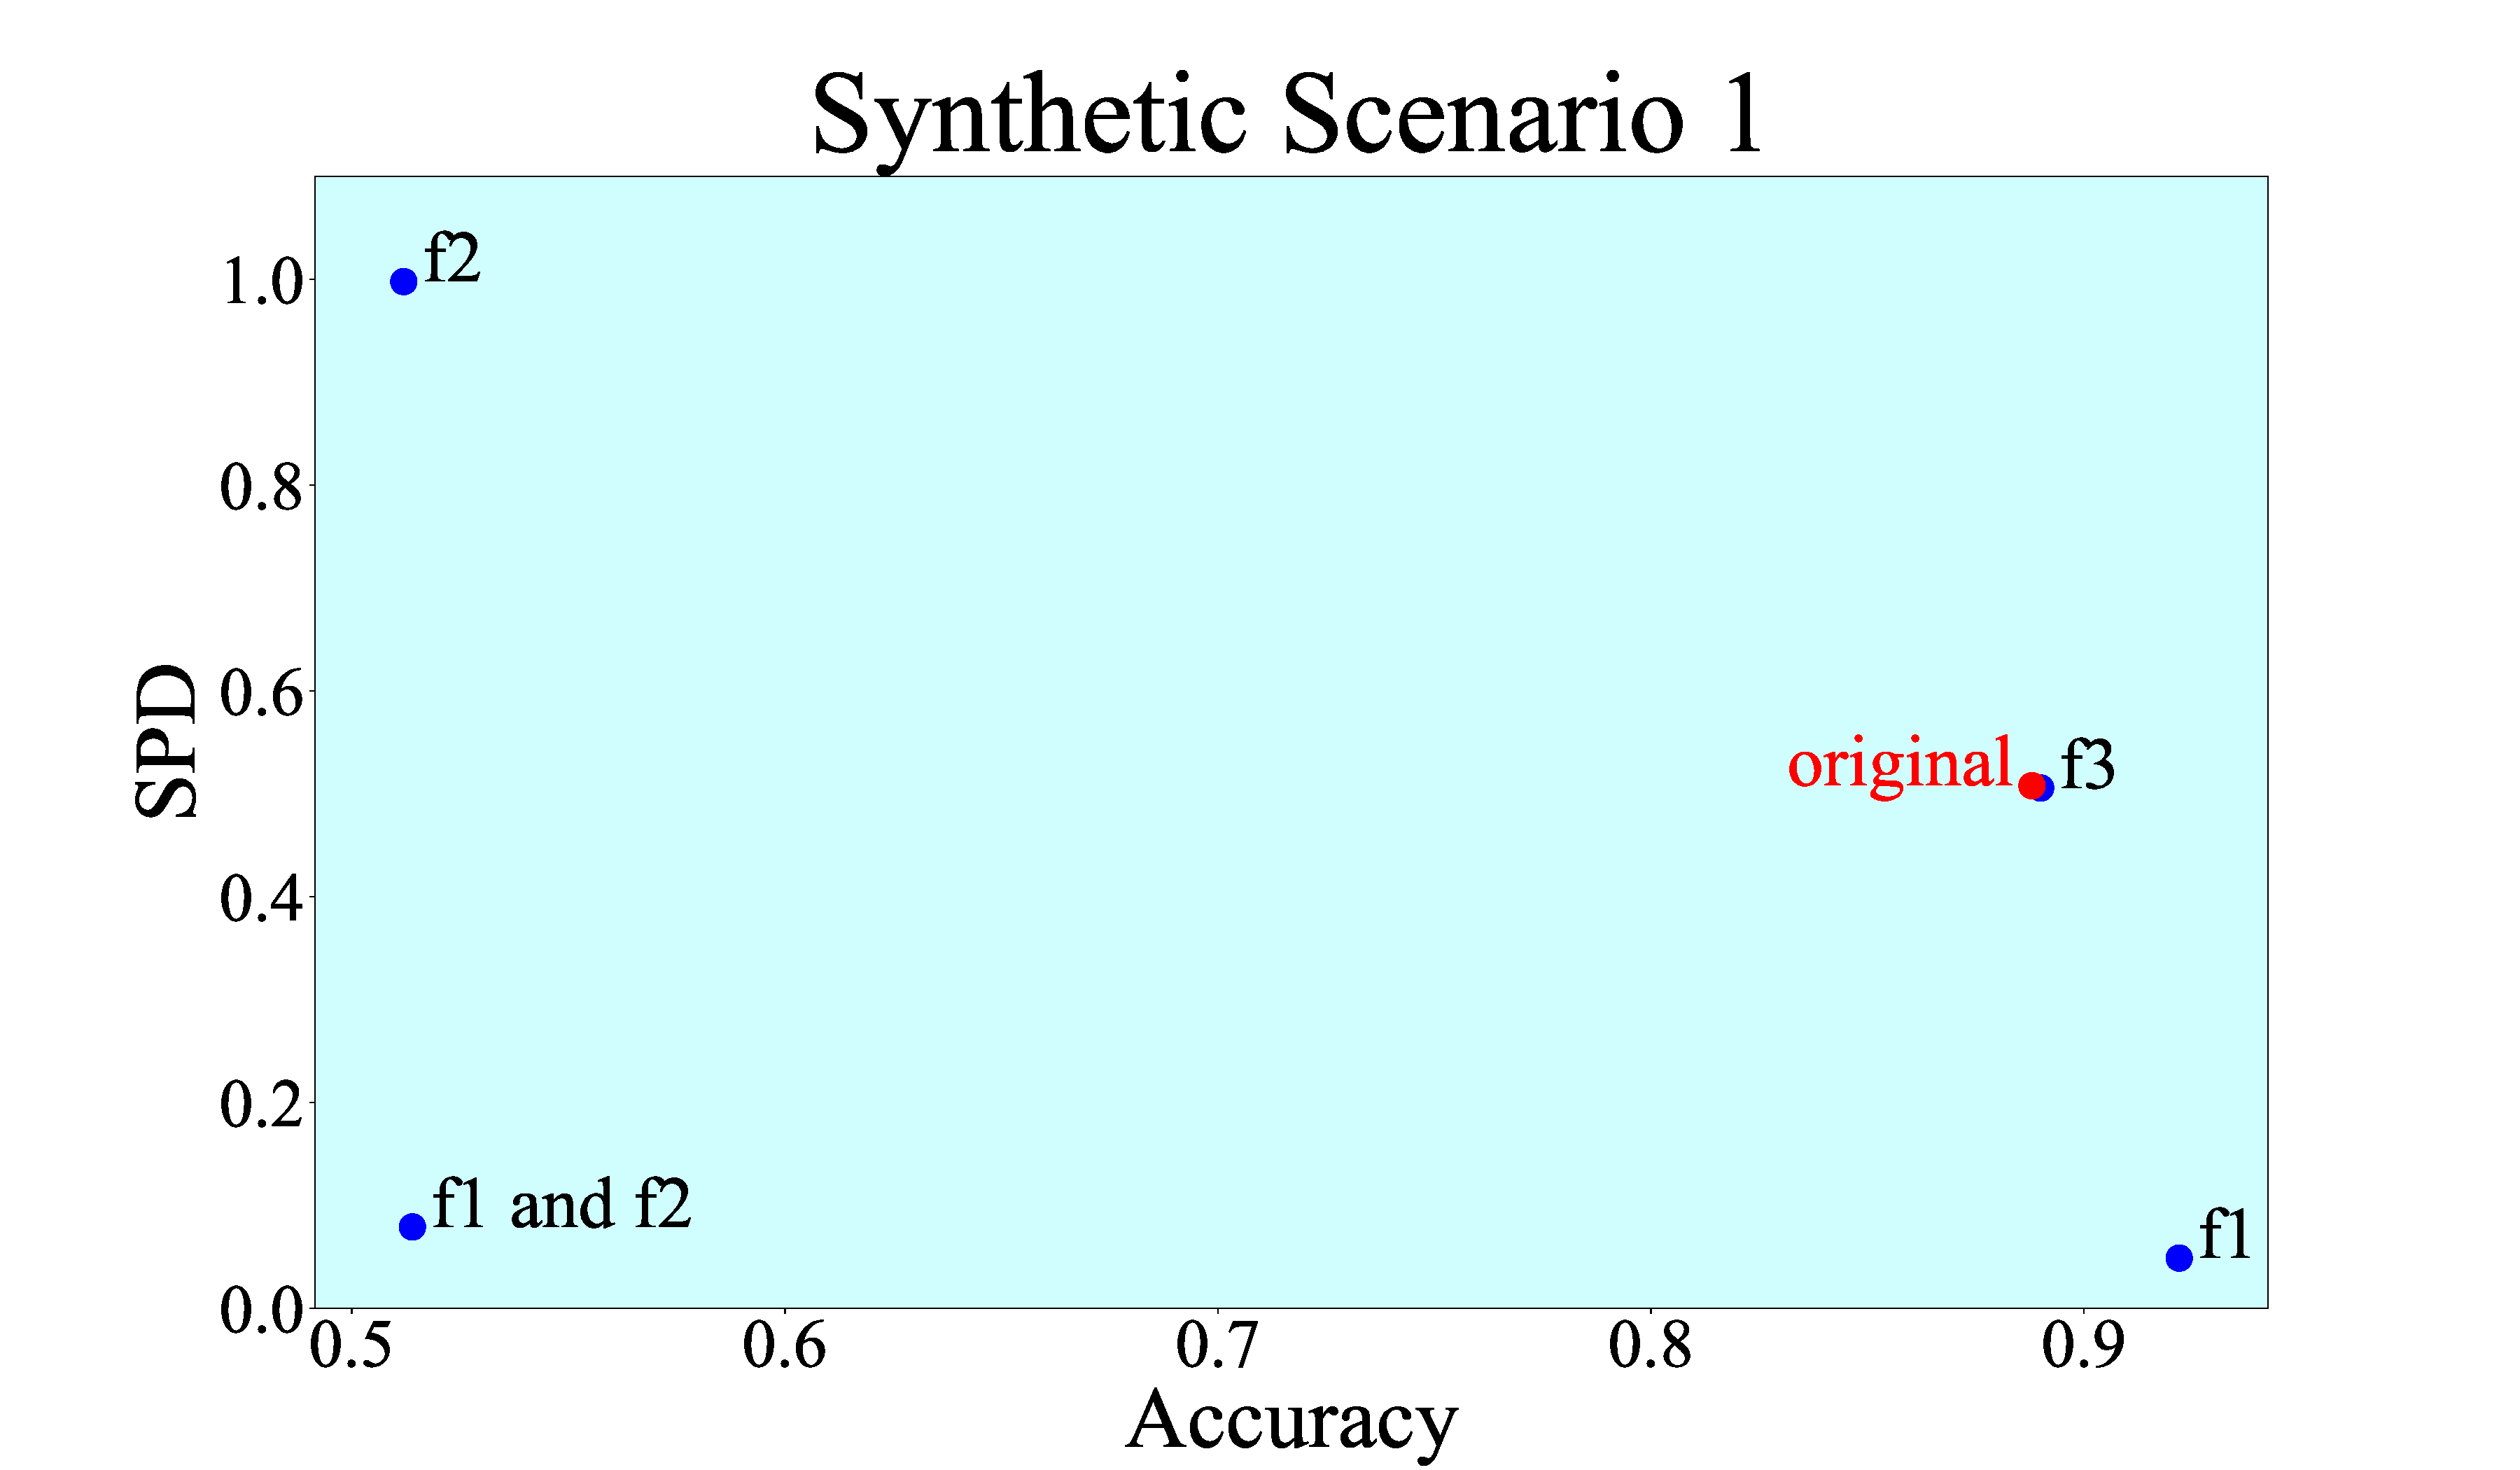
\includegraphics[width=\textwidth,trim=2.5cm 0cm 4.5cm 1.0cm,clip=true]{./images/inter_imgs/no_err_newscen1.pdf}
\end{subfigure}
\begin{subfigure}[b]{0.5\textwidth}
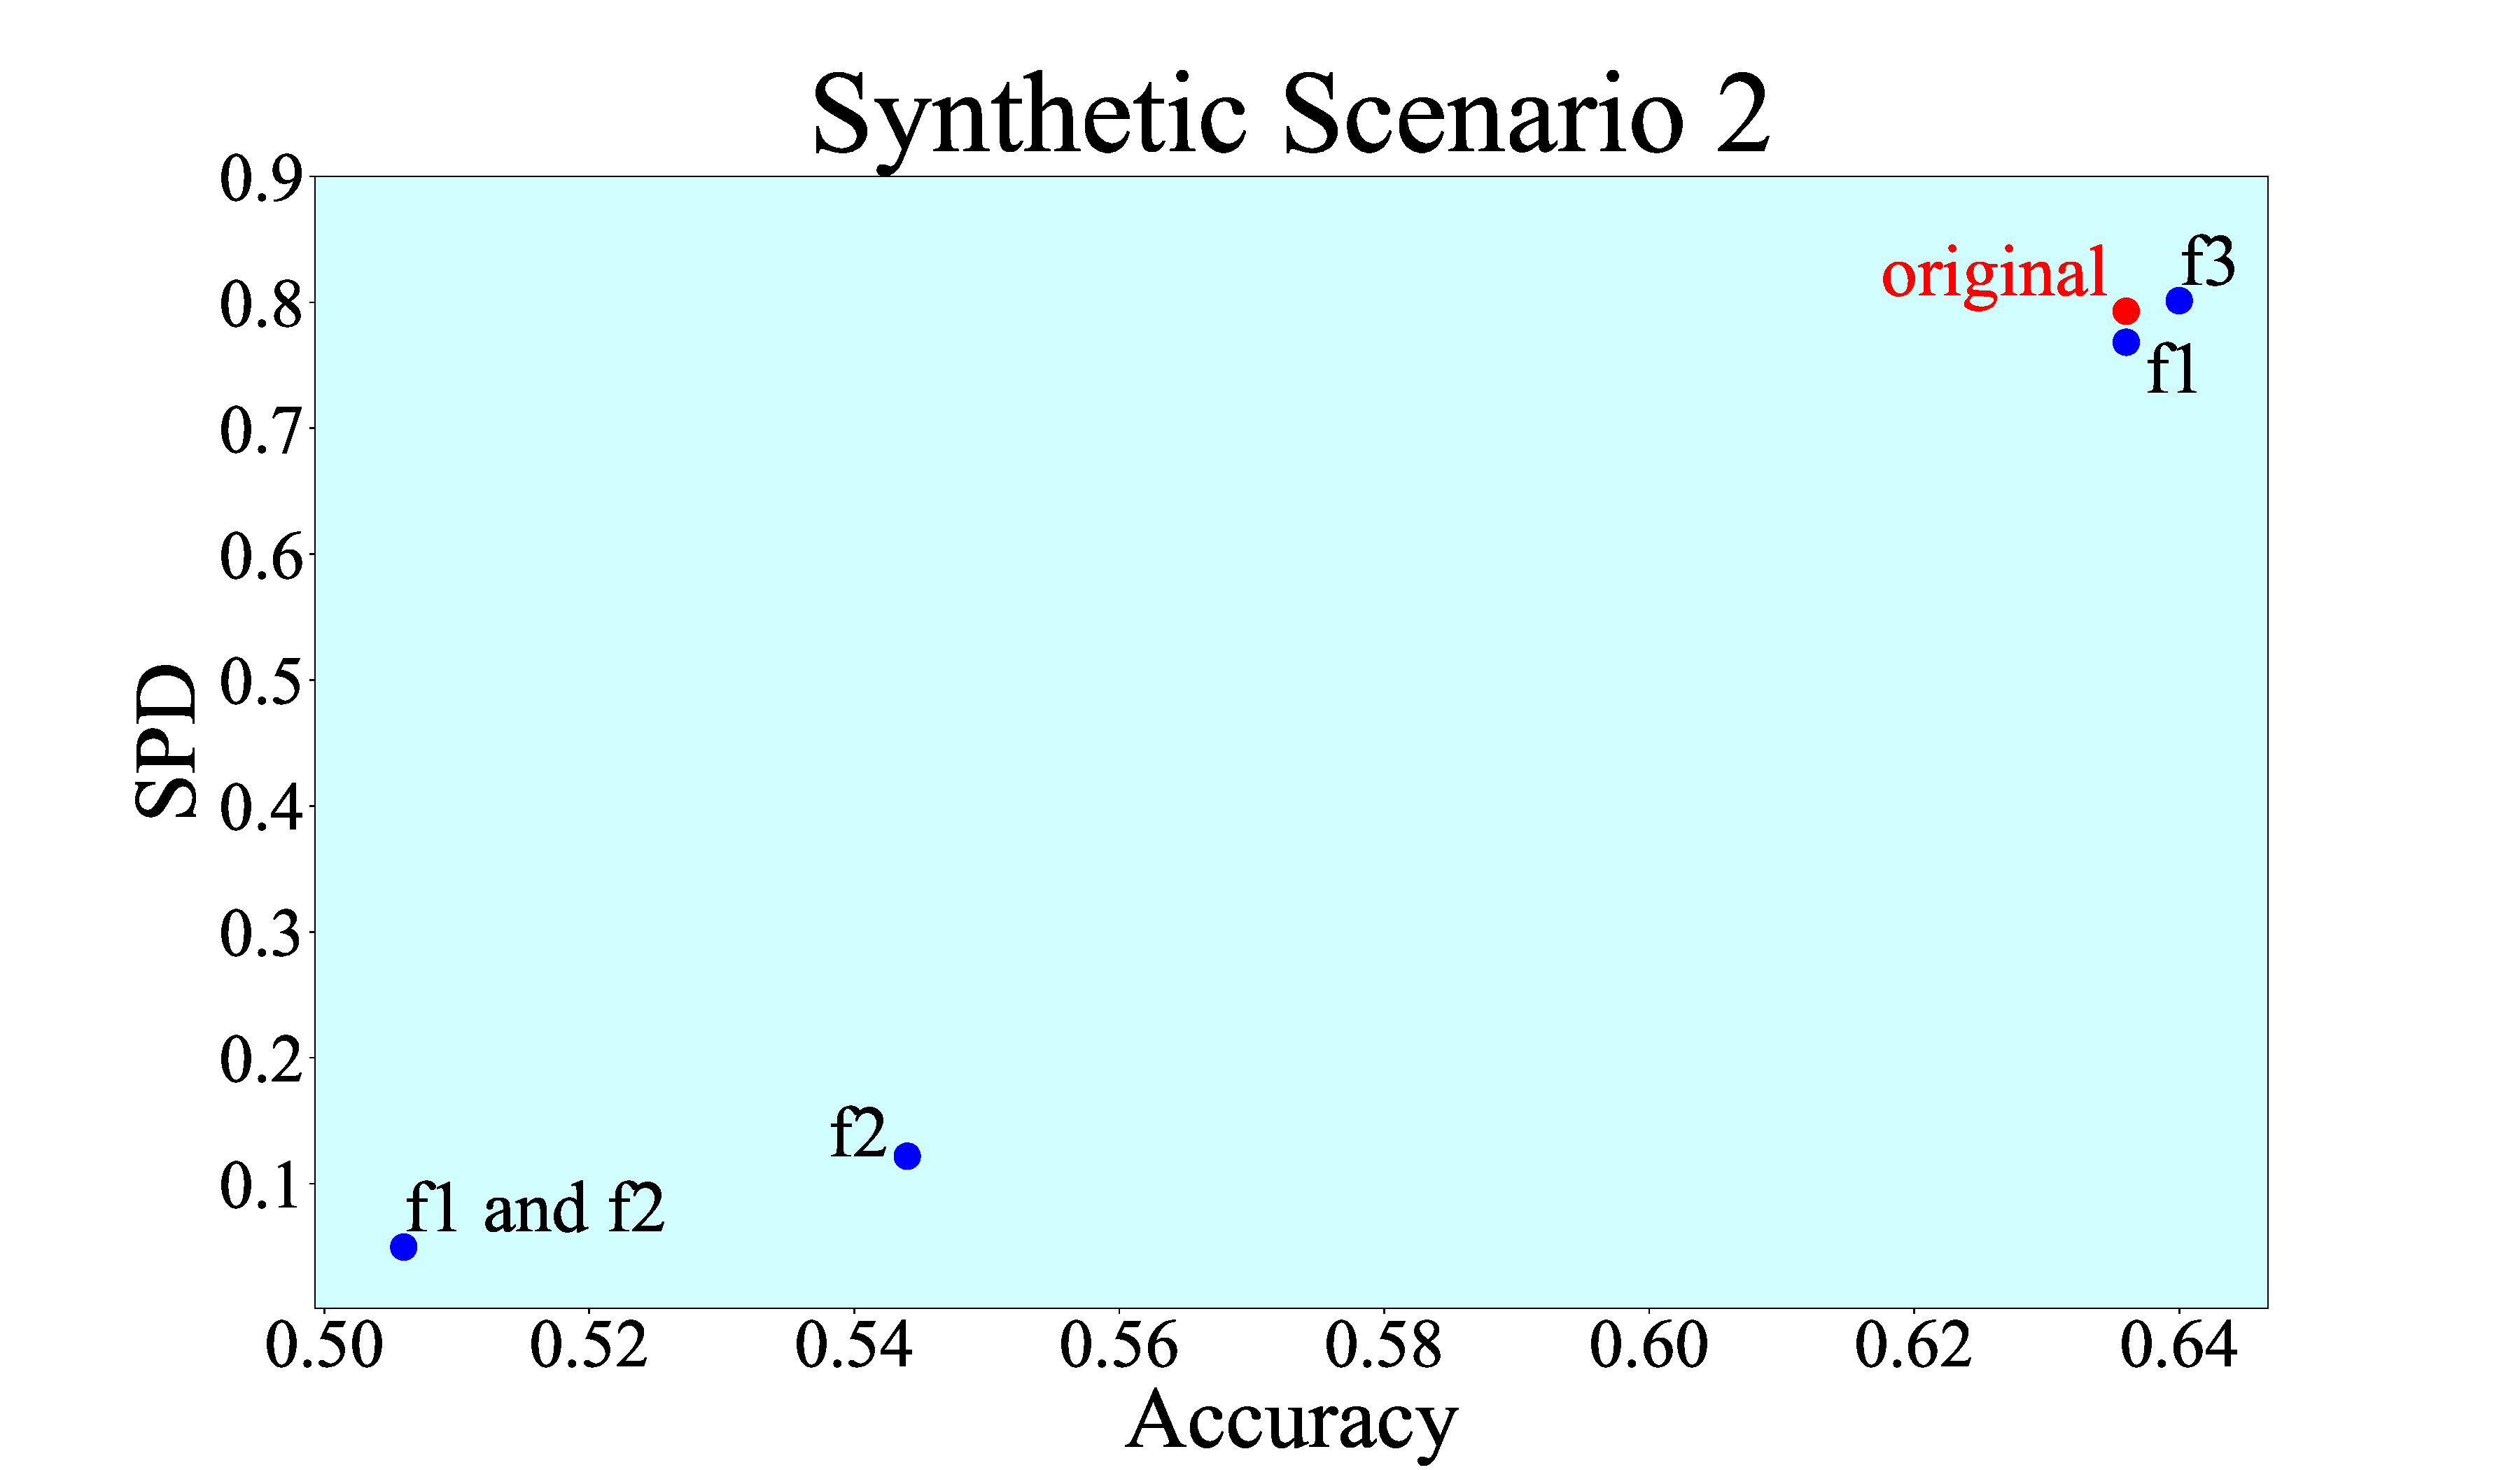
\includegraphics[width=\textwidth,trim=2.5cm 0cm 4.5cm 1.0cm,clip=true]{./images/inter_imgs/no_err_newscen2.pdf}
\end{subfigure}
\begin{subfigure}[b]{0.5\textwidth}
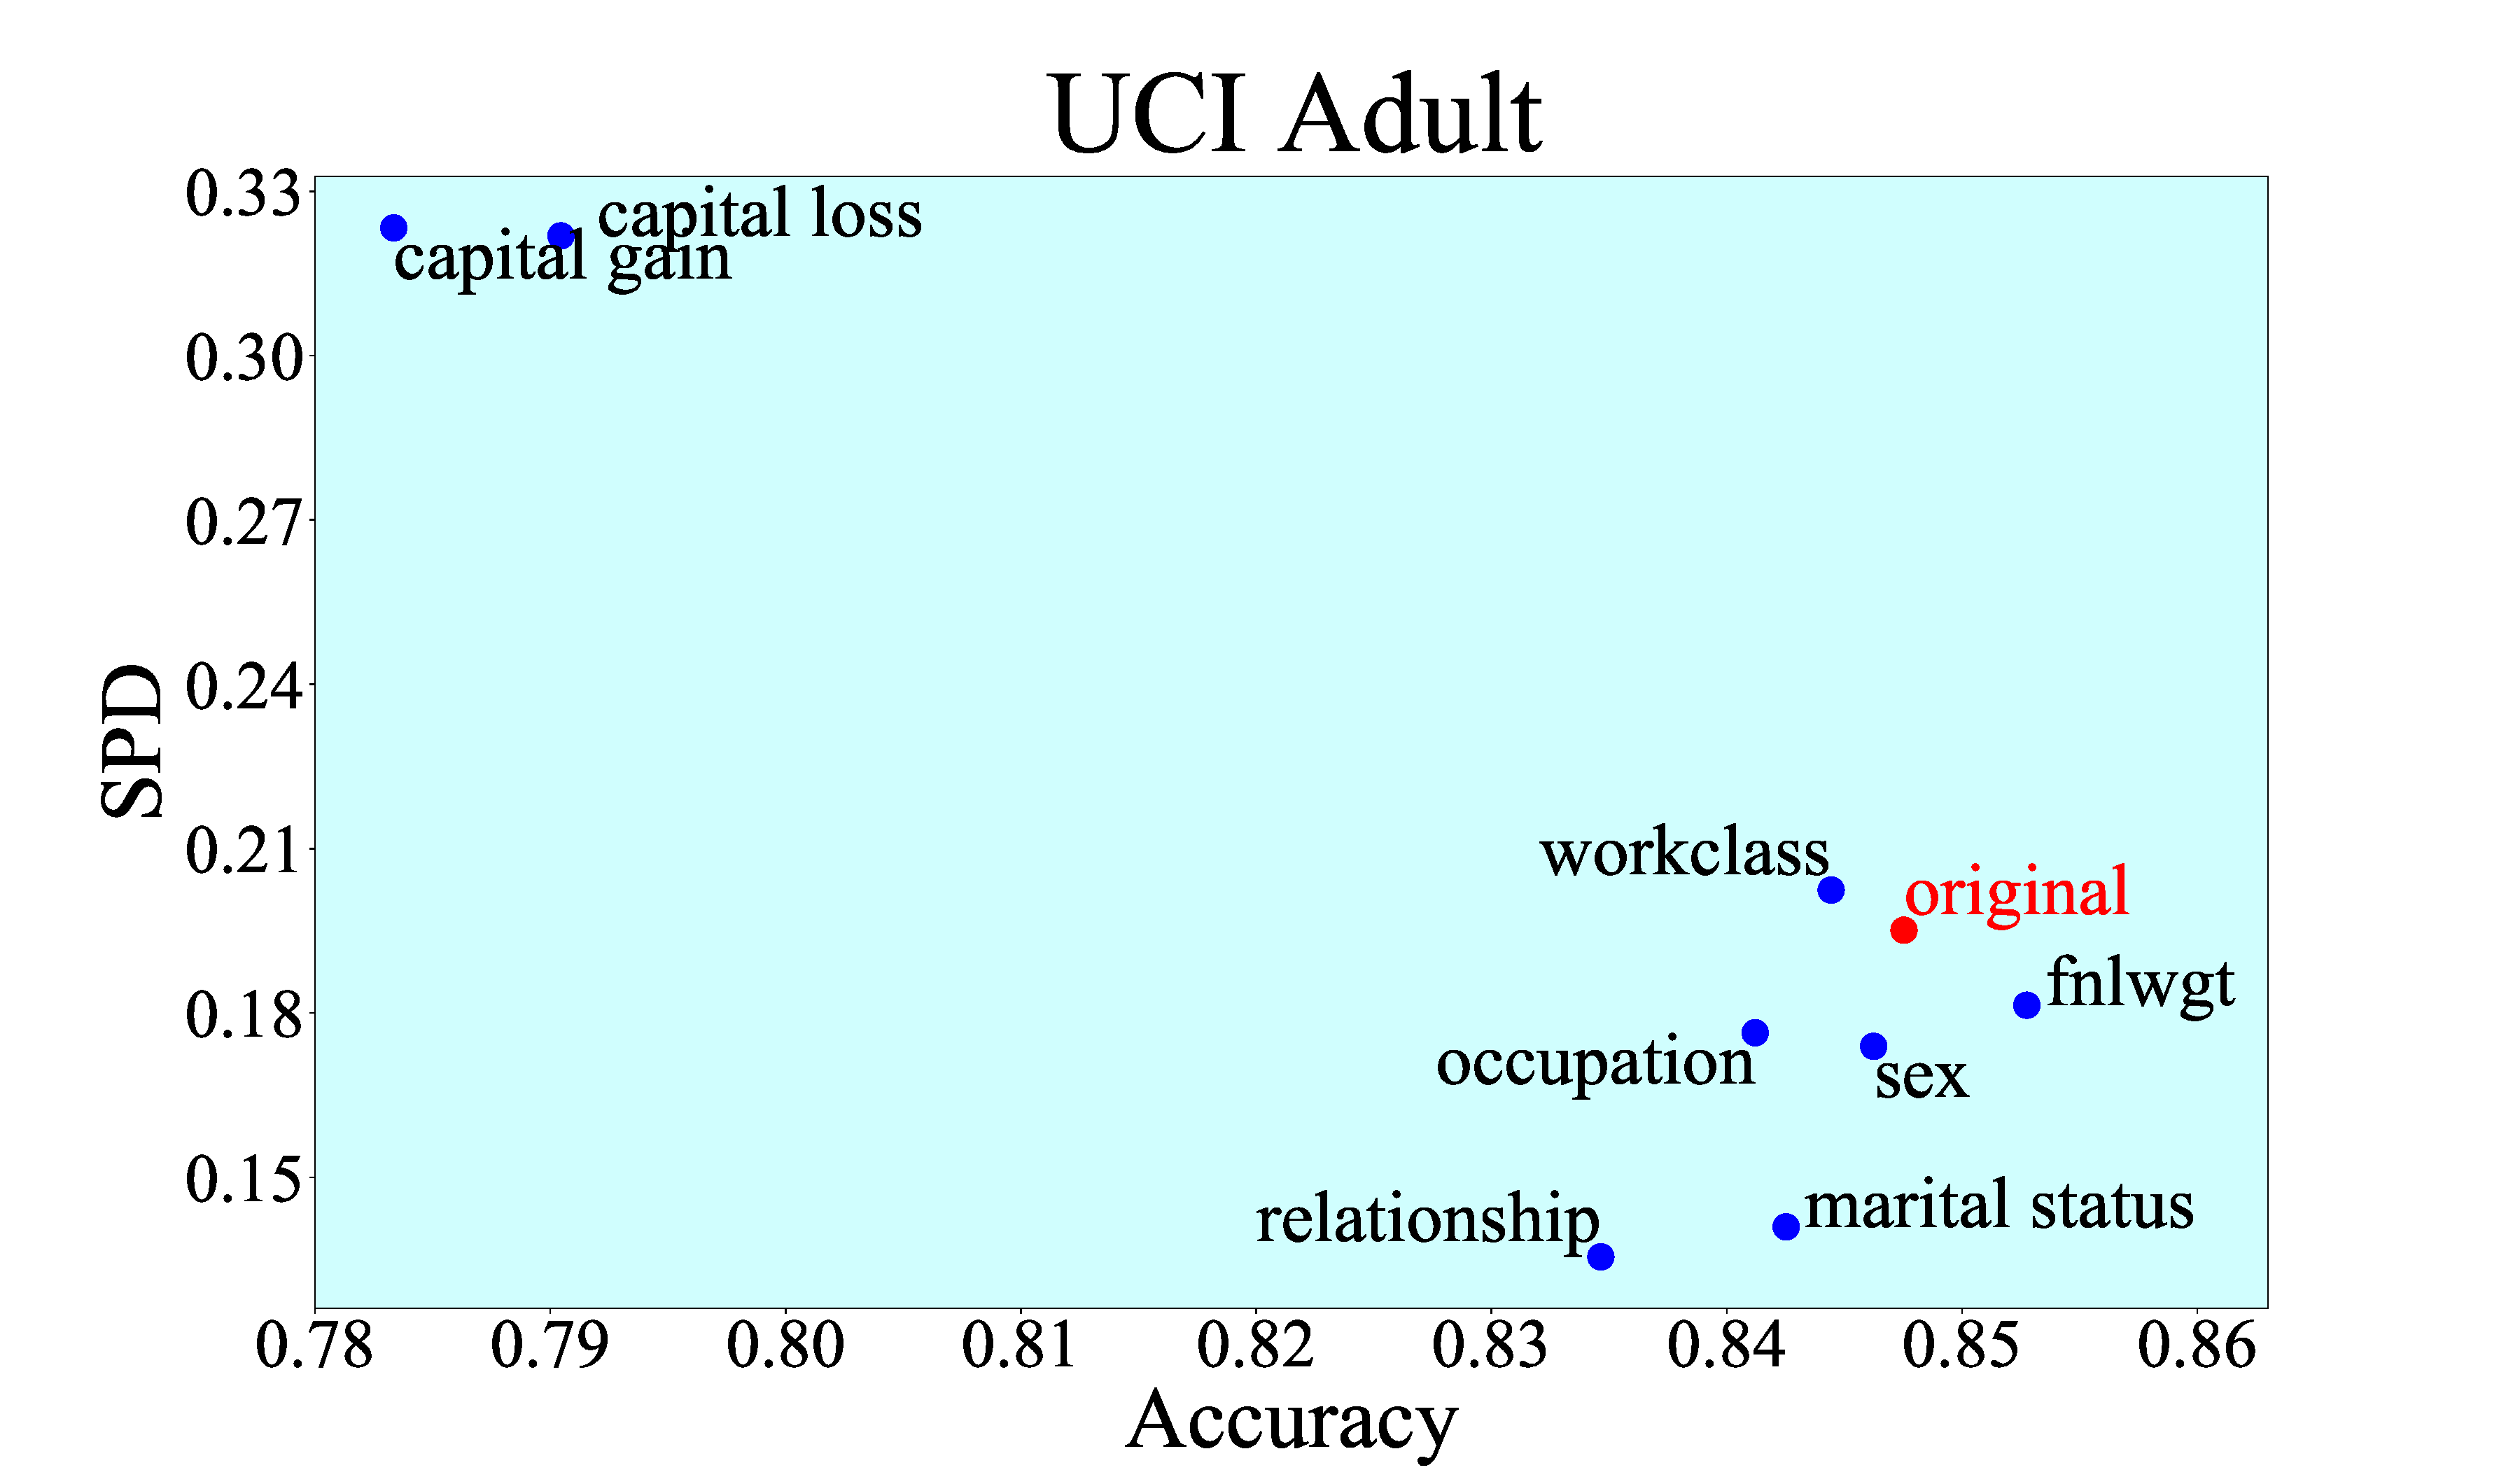
\includegraphics[width=\textwidth,trim=2.5cm 0cm 4.5cm 1.0cm,clip=true]{./images/inter_imgs/no_err_real_data_adult_subset2.pdf}
\end{subfigure}
\begin{subfigure}[b]{0.5\textwidth}
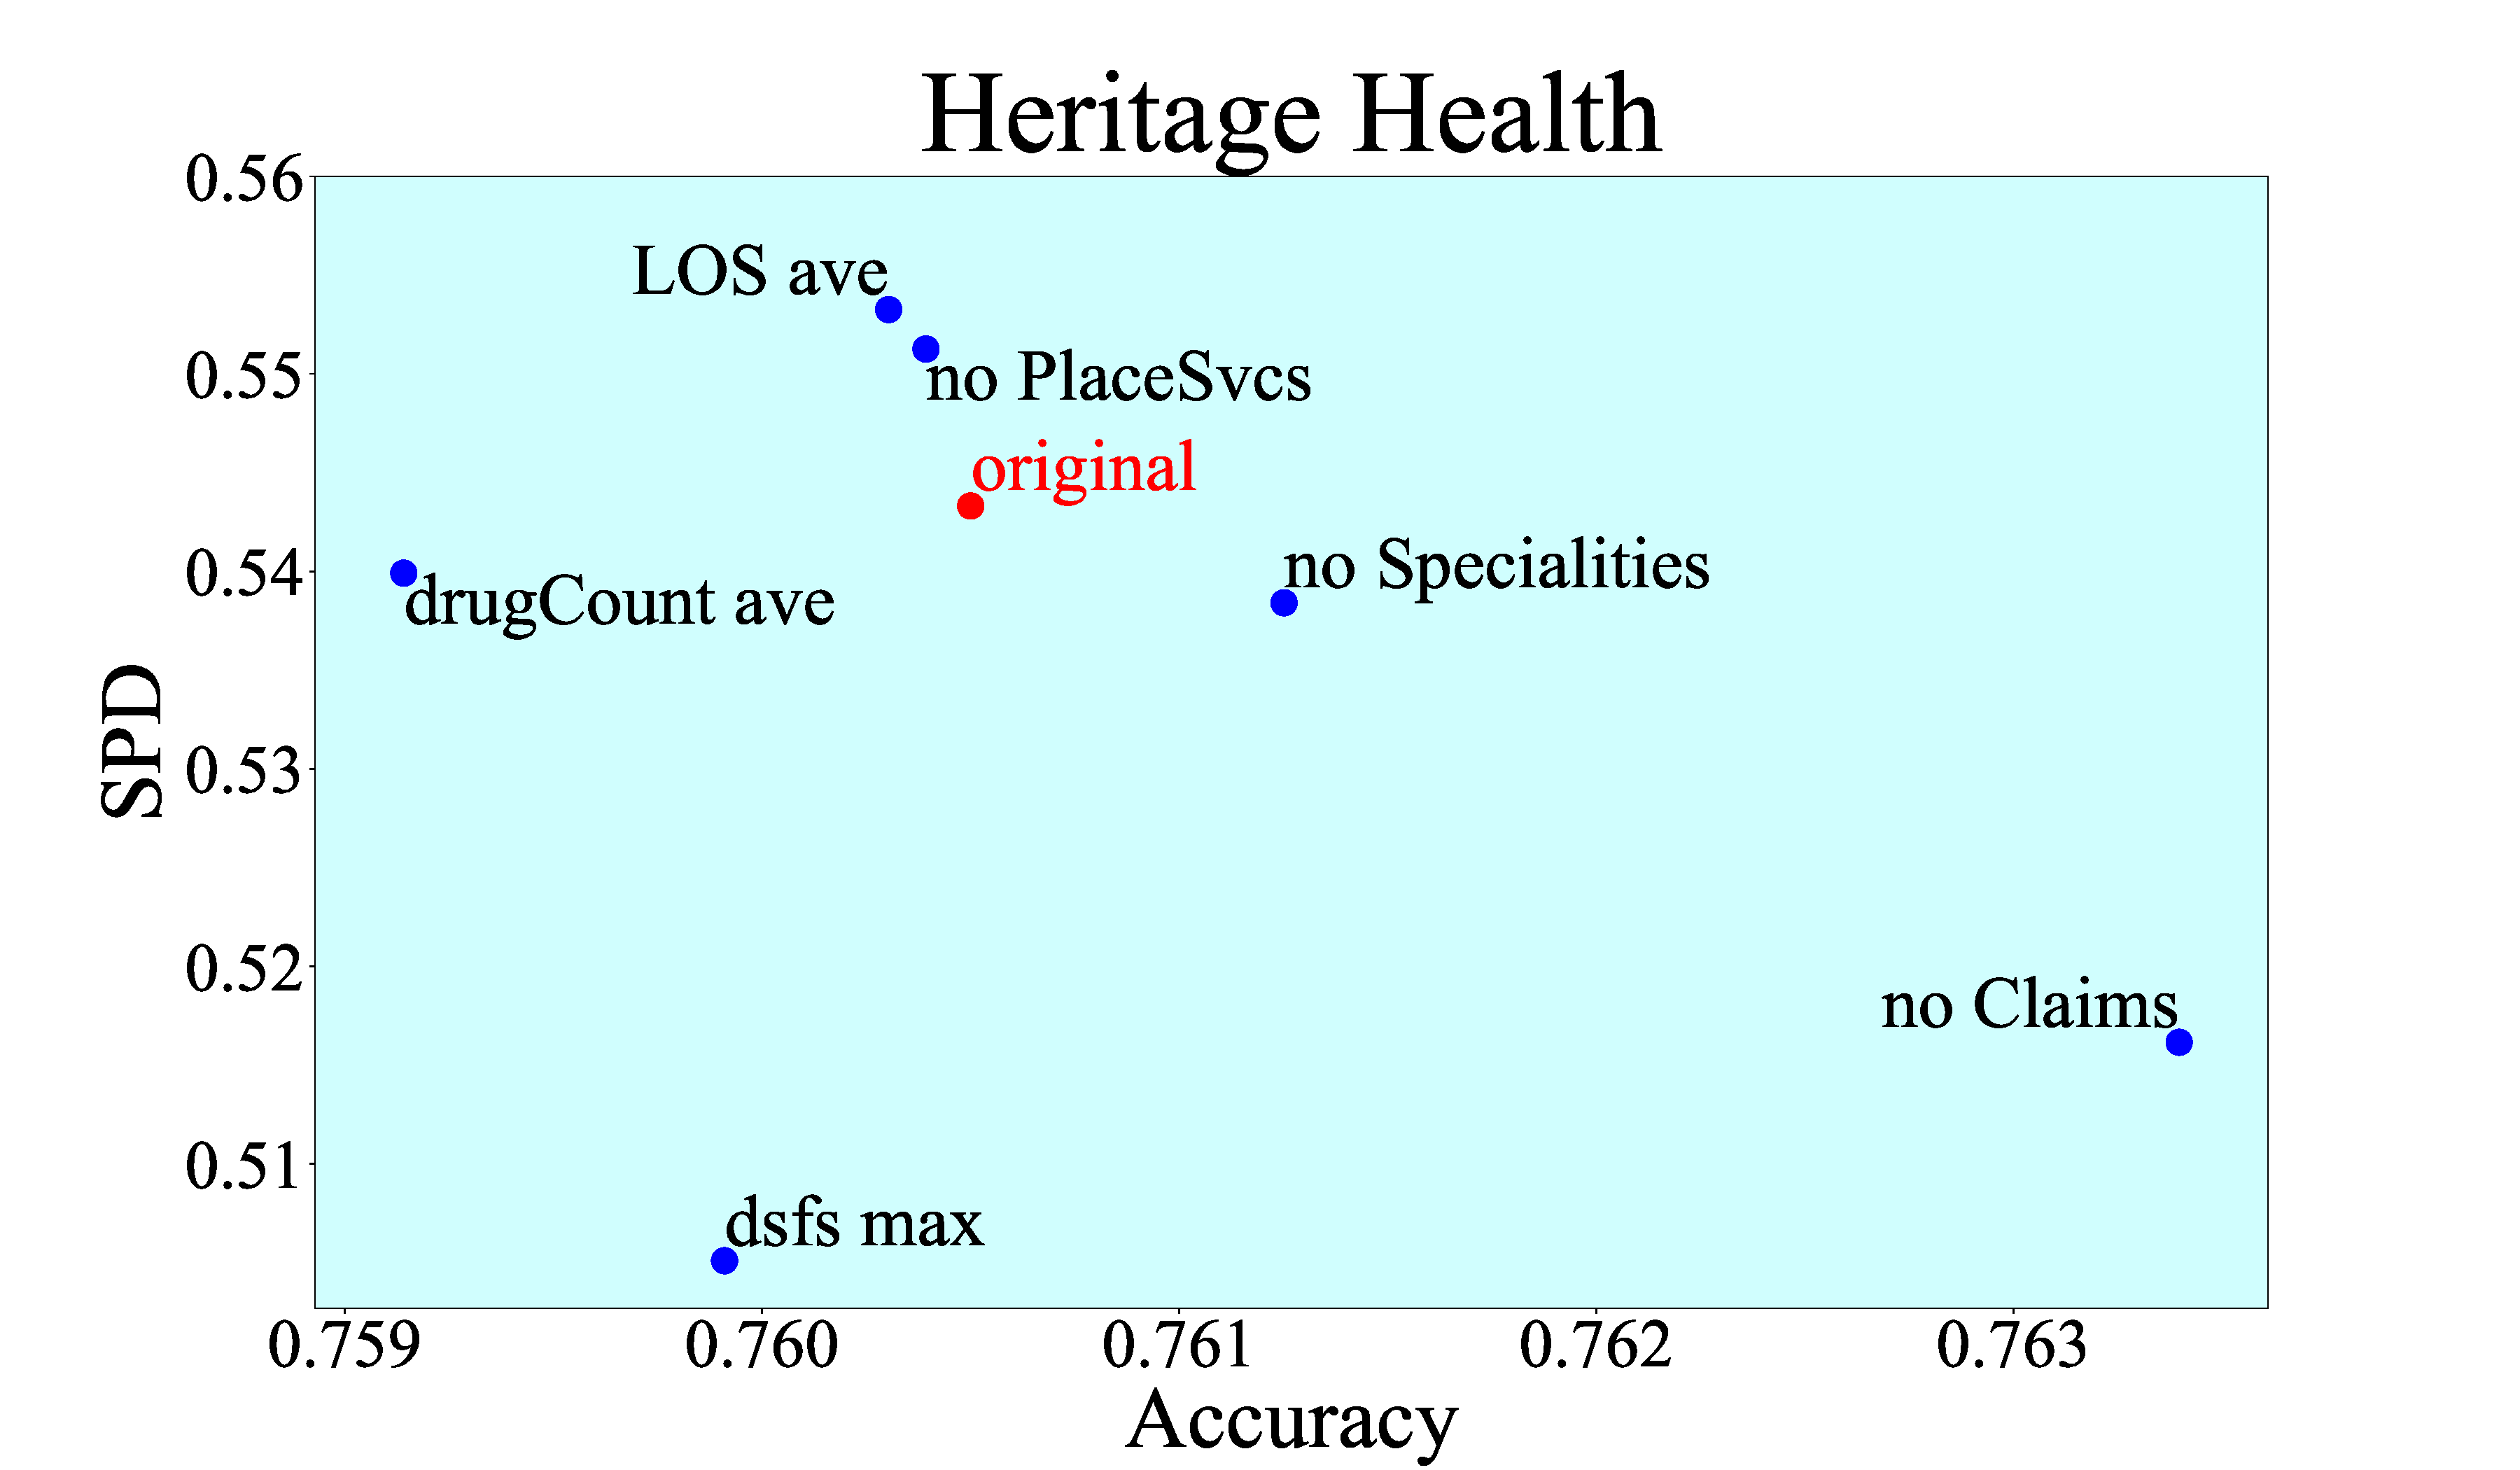
\includegraphics[width=\textwidth,trim=2.4cm 0cm 4.5cm 1.0cm,clip=true]{./images/inter_imgs/no_err_real_data_health_subset2.pdf}
\end{subfigure}
\caption{Results from the synthetic datasets on top and real-world datasets in the bottom. Labels on the points represent the feature name that was removed. The results show how the accuracy and fairness of the model (in terms of statistical parity difference) change by exclusion of each feature. The red original point represents the results of the model including all the features.}
\label{fig:interpret_results}
\end{figure*}
% \begin{figure*}[t]
% \begin{subfigure}[b]{0.5\textwidth}
% 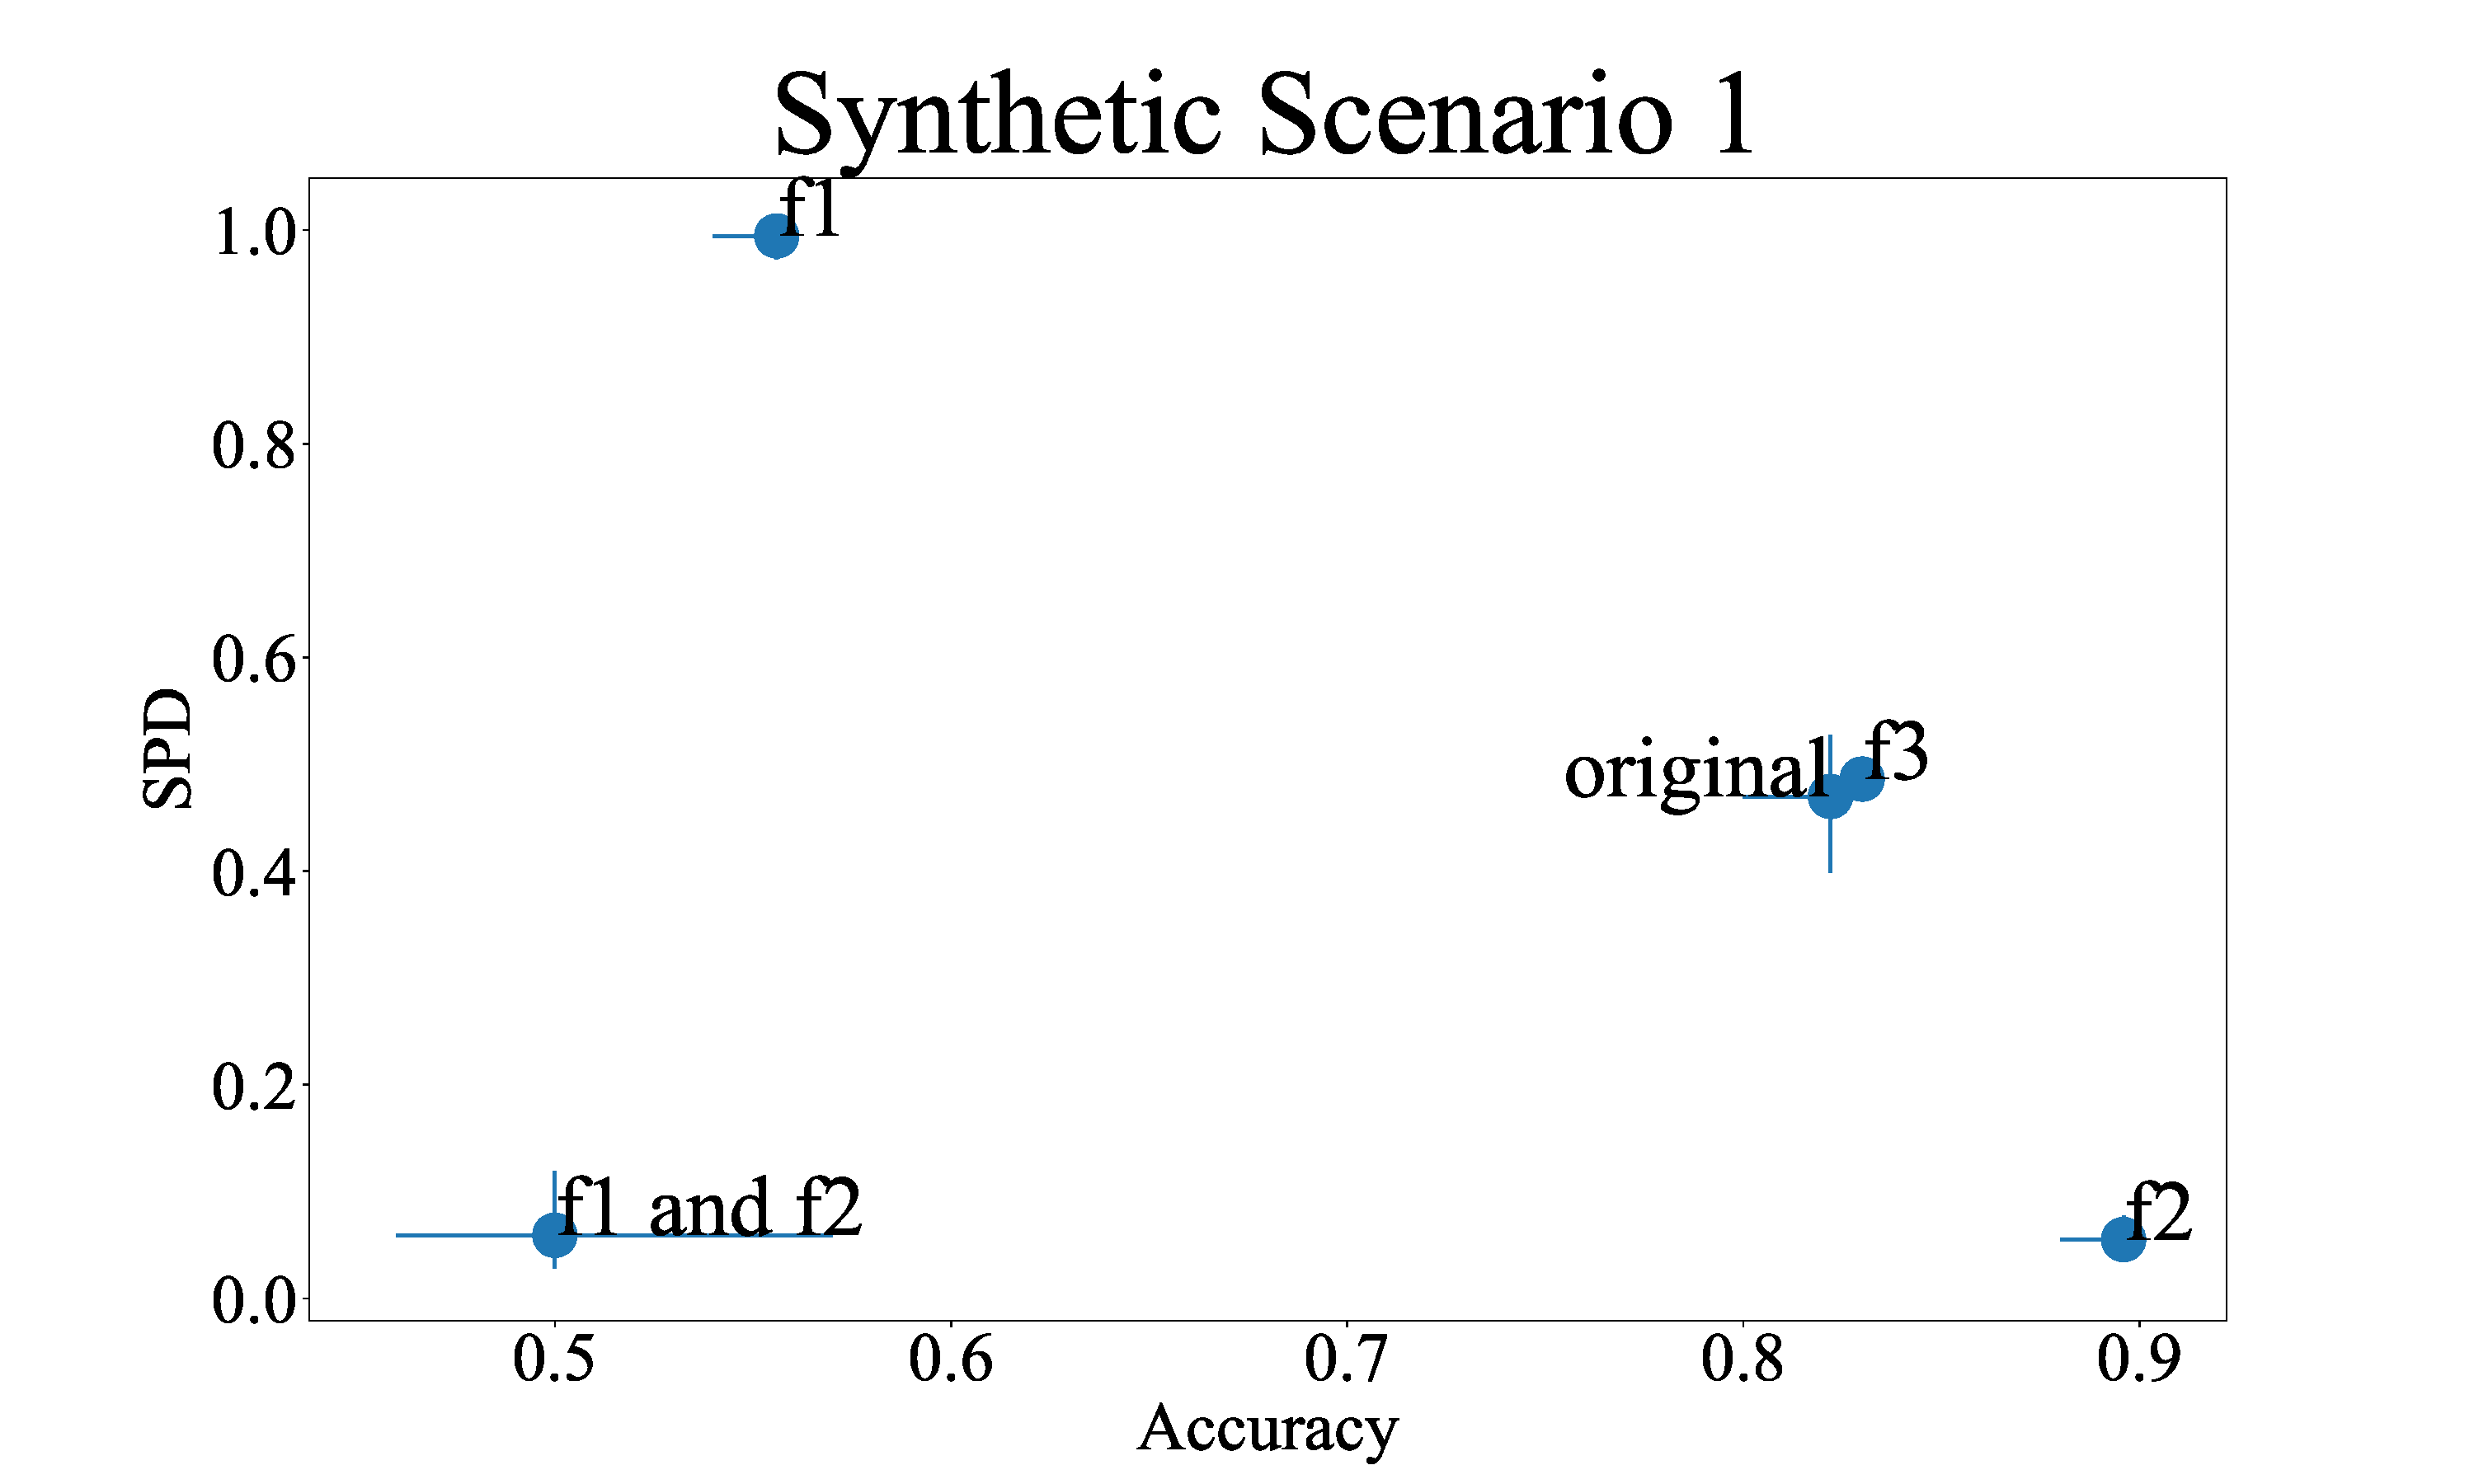
\includegraphics[width=\textwidth,trim=2.5cm 0.5cm 2.5cm 0.8cm,clip=true]{./images/inter_imgs/newscen1.pdf}
% \end{subfigure}
% \begin{subfigure}[b]{0.5\textwidth}
% 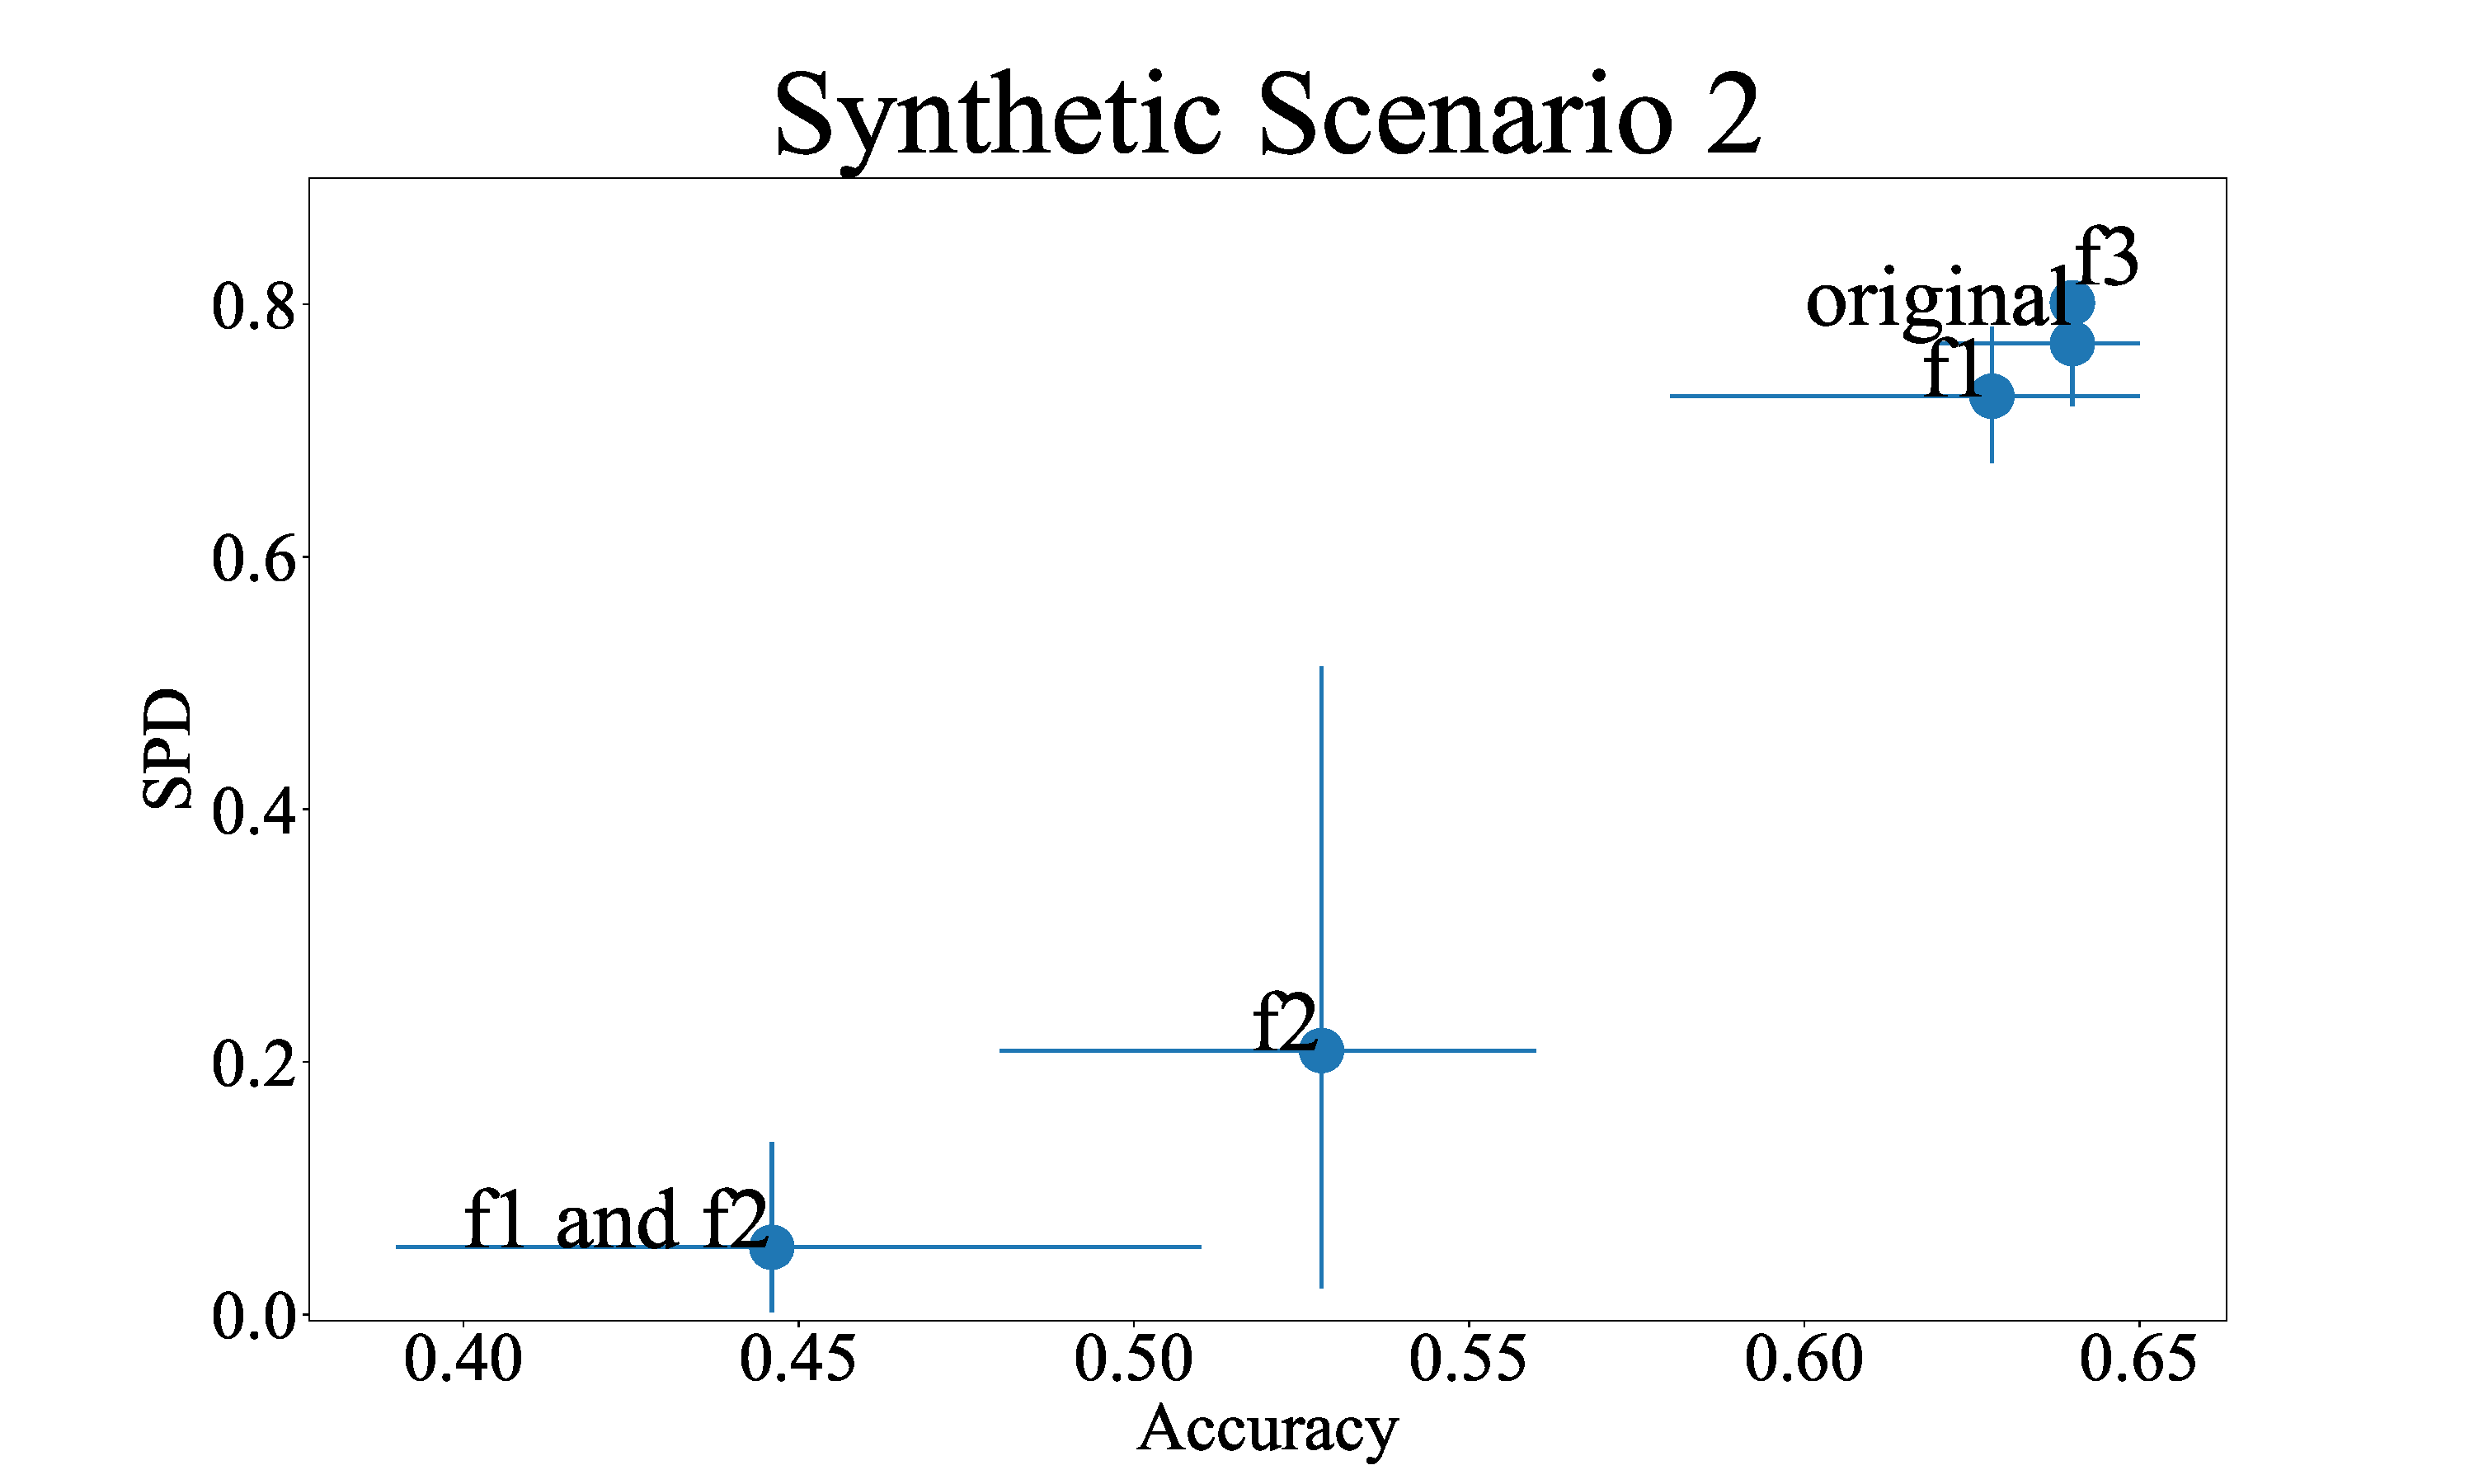
\includegraphics[width=\textwidth,trim=2.5cm 0.5cm 2.5cm 0.8cm,clip=true]{./images/inter_imgs/newscen2.pdf}
% \end{subfigure}
% \begin{subfigure}[b]{0.5\textwidth}
% 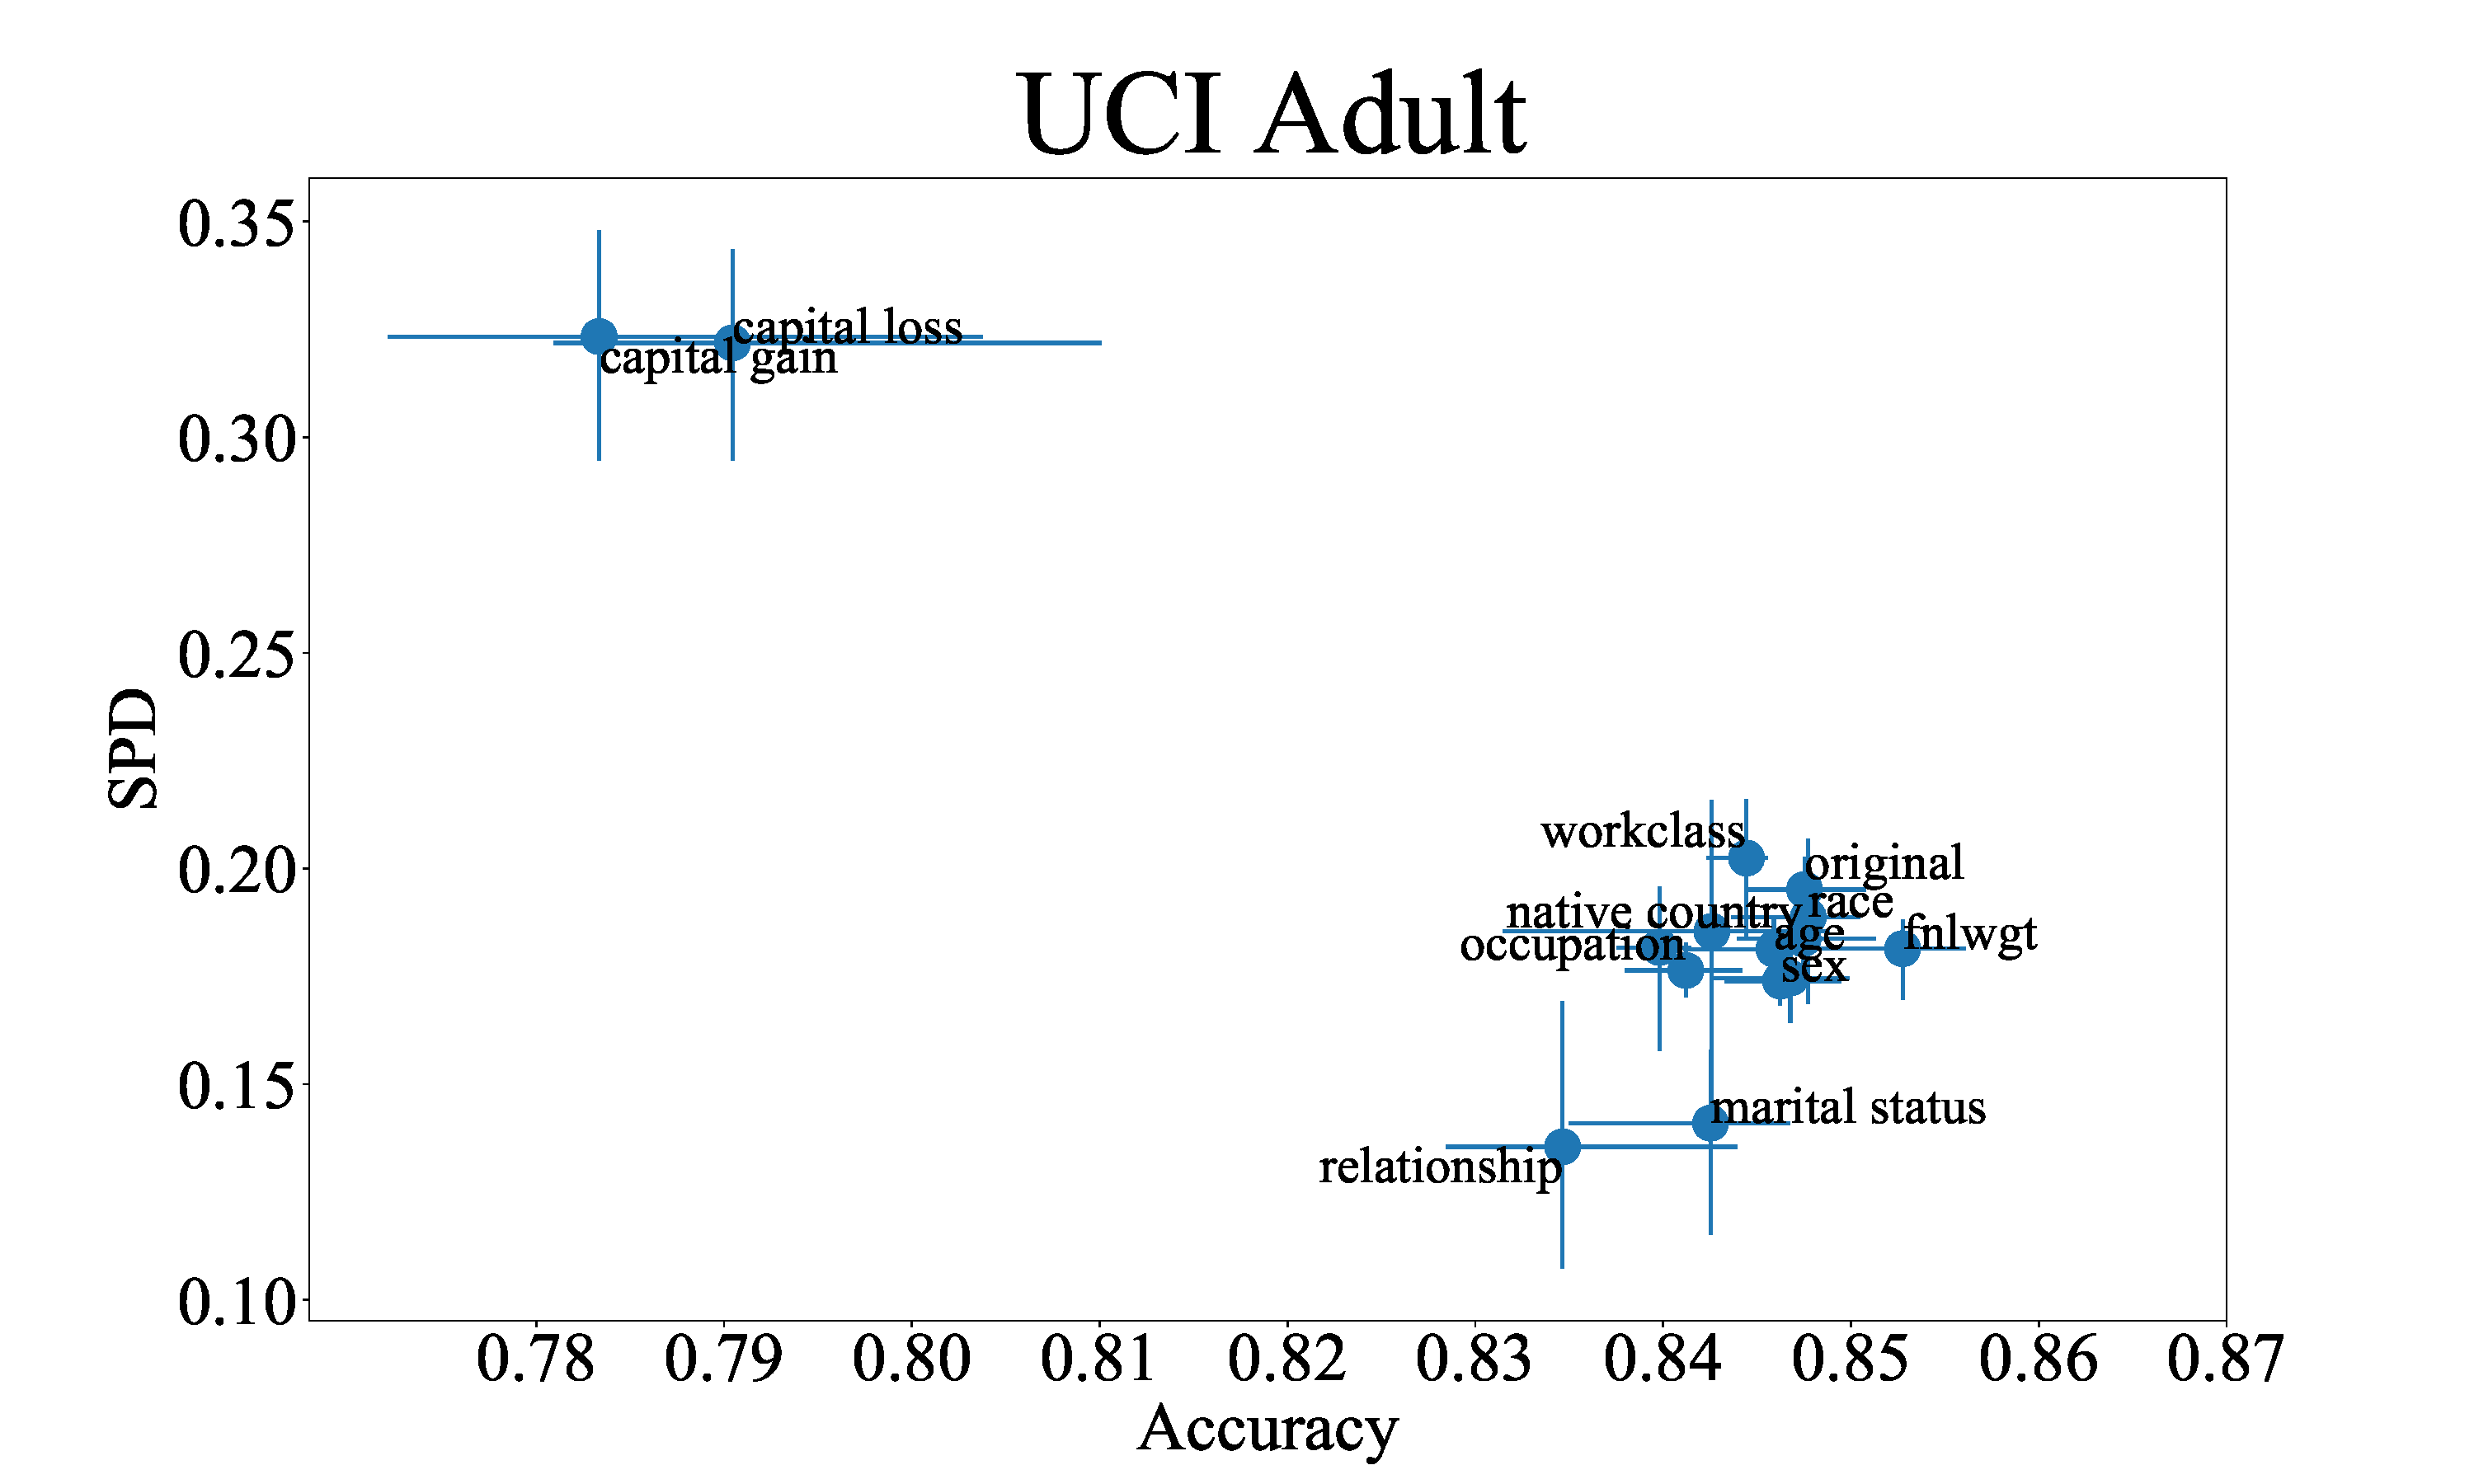
\includegraphics[width=\textwidth,trim=2.5cm 0.5cm 2.5cm 0.8cm,clip=true]{./images/inter_imgs/real_data_adult2.pdf}
% \end{subfigure}
% \begin{subfigure}[b]{0.5\textwidth}
% 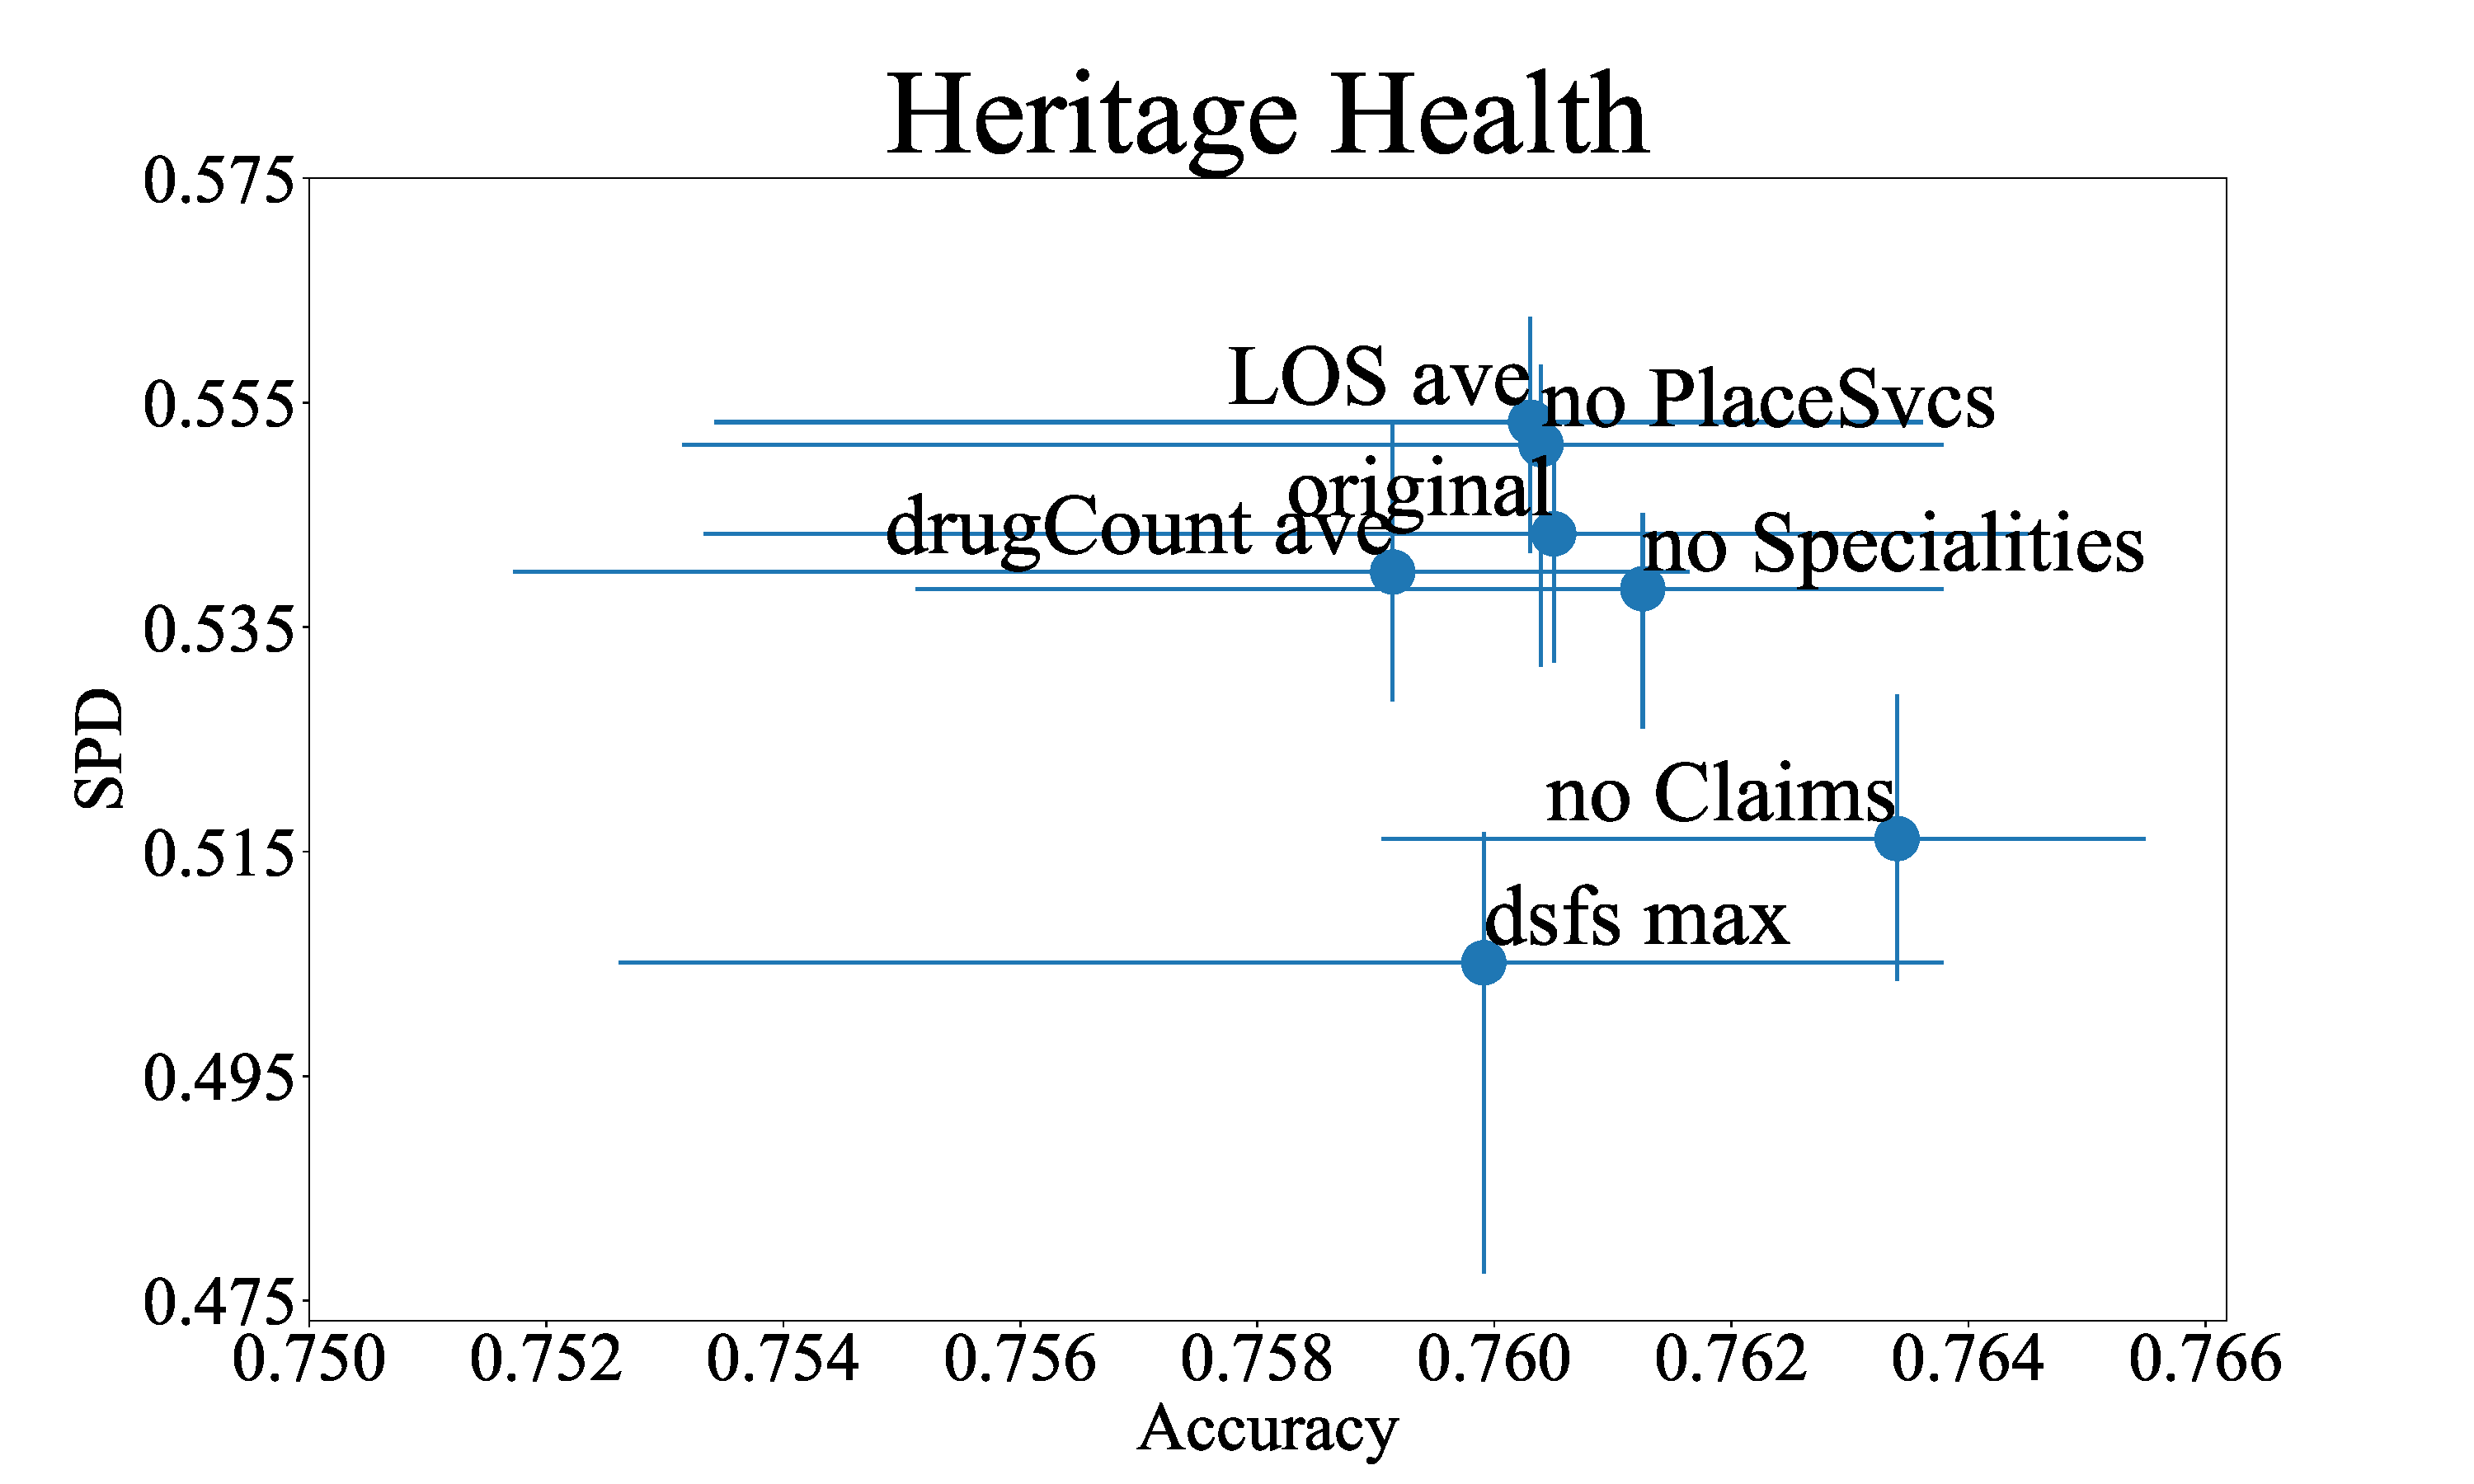
\includegraphics[width=\textwidth,trim=2.5cm 0.5cm 2.5cm 0.8cm,clip=true]{./images/inter_imgs/real_data_health_subset2.pdf}
% \end{subfigure}
% \caption{Results from the synthetic datasets on top and real-world datasets in the bottom. Labels on the points represent the feature name that was removed. The results show how the accuracy and fairness of the model (in terms of statistical parity difference) change by exclusion of each feature. The red original point represents the results of the model including all the features.}
% \label{interpret_results}
% \end{figure*}


First, we validate that our interpretability framework can capture correct attributions by controlled experiments with synthetic data. We also experiment with \textit{UCI Adult} and \textit{Heritage Health} and argue that the captured attributions are reasonable. Fig.~\ref{fig:interpret_results} summarizes our results. The interpretability framework correctly captures the intentional behavior created in the synthetic datasets.

In \textit{Scenario 1}, as expected, $f_2$ is correctly attributed to being responsible for the accuracy, and removing it hurts the accuracy drastically. Similarly, $f_1$ is correctly shown to be responsible for unfairness, and removing it creates a fairer outcome. Ideally, the model should not be using any information about $f_1$ as it is independent of the task, but it does. Therefore, by removing $f_1$, we can be sure that information is not used and hence outcomes are fair. Lastly, as expected, $f_3$ was the irrelevant feature, and its effects on accuracy and fairness are negligible. Another interesting observation is that $f_2$ is helping the model achieve fairness since its exclusion means that the model should rely on $f_1$ for decision making, resulting in more bias; thus, removing $f_2$ harms accuracy and fairness as expected.

In \textit{Scenario 2}, our framework captures the effect of indirect discrimination. We can see that removing $f_2$  reduces bias as well as accuracy drastically. This is because $f_2$ is the predictive feature, but due to its correlation with $f_1$, it can also indirectly affect the model's fairness. More interestingly, although $f_1$ is the sensitive feature, removing it does not play a drastic role in fairness or the accuracy. This is an important finding as it shows why removing $f_1$ on its own can not give us a fairer model due to the existence of correlations to other features and indirect discrimination. 
% Thus, our framework recognize such behavior and help design better mitigation strategies targeted towards responsible features which will lead us to our mitigation strategy discussed in the next section.

Lastly, Fig.~\ref{fig:interpret_results}, also shows results on a subset of the features from the \textit{UCI Adult} and \textit{Heritage Health} datasets (To keep the plots uncluttered and readable, we incorporated the most interesting features in the plot). These  can provide us with some intuition about how different features in these datasets contribute to the fairness and accuracy of the model. While features such as capital gain and capital loss in the \textit{UCI Adult} dataset are responsible for improving accuracy and reducing bias, we can observe from the results in  Fig.~\ref{fig:interpret_results} that features such as relationship or marital status that can be directly or indirectly correlated with sex are causing unfairness. These results are intuitive and once again confirm the reliability of our framework.
% Sex was used as the sensitive feature in the Adult dataset and age in the Heritage Health dataset.
% \todo{(We should talk more about how the attributions are correct or intuitive, using one or two examples from the figure. We should also point to some of the results in the appendix. Nina: If space is left we can do this...)}

%From the results, we conclude that attention weights capture the true and expected behavior and that this framework can provide reliable attributions for fairness and accuracy of the model.
The above results validate that attention weights capture the true or the expected behavior and that this framework can provide reliable attributions for the fairness and accuracy of the model.

\vspace{-0.3cm}
\subsection{Attention as a Mitigation Technique}
\vspace{-0.3cm}
\begin{figure*}[t]
    \begin{subfigure}[b]{0.49\textwidth}
        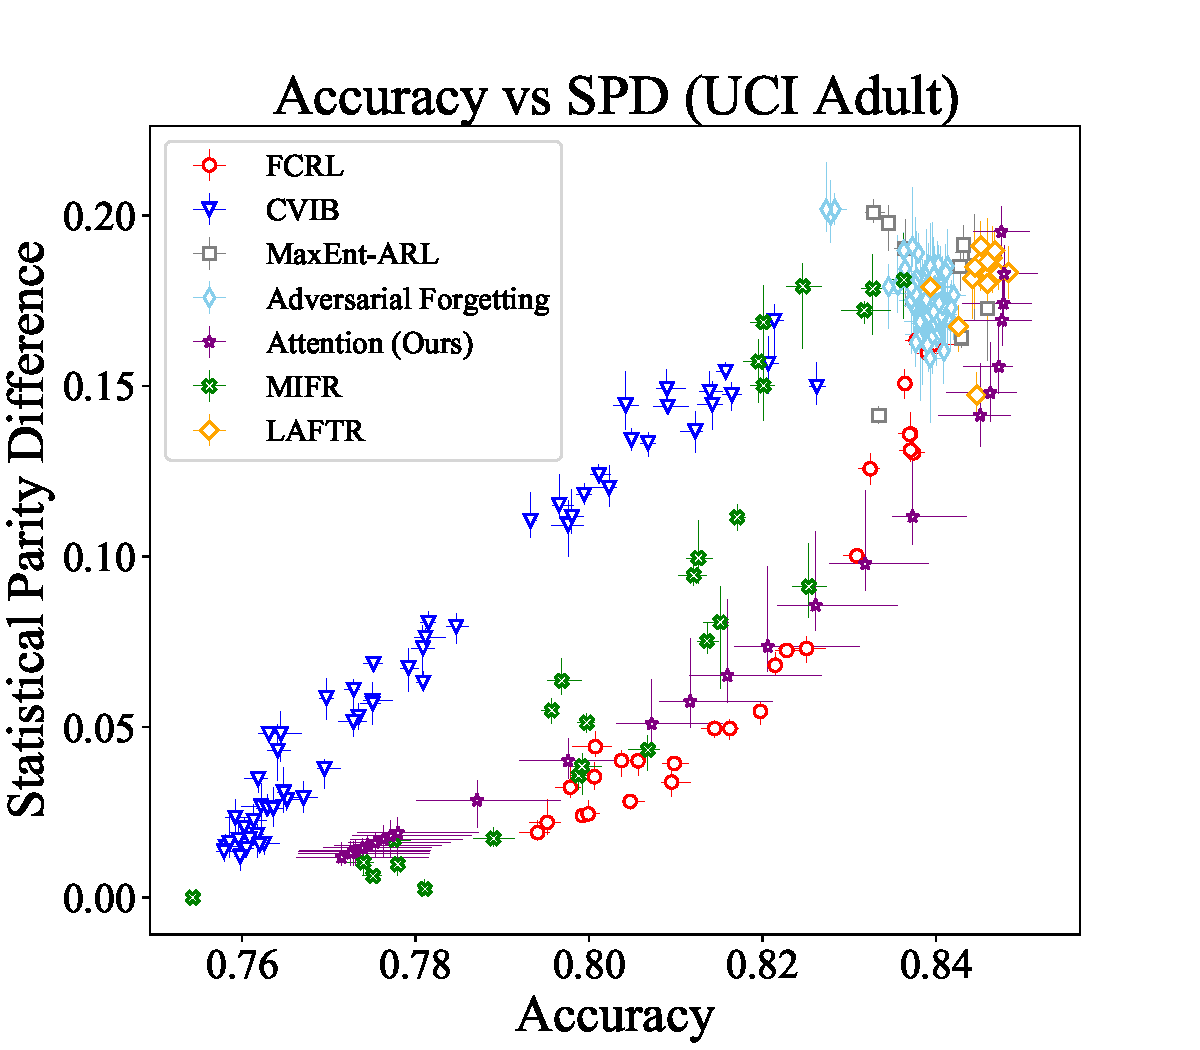
\includegraphics[width=\textwidth,trim=0cm 0cm 1.8cm 1.0cm,clip=true]{./images/mitig_imgs/adult_results_err.pdf}
    \end{subfigure}
    \begin{subfigure}[b]{0.49\textwidth}
        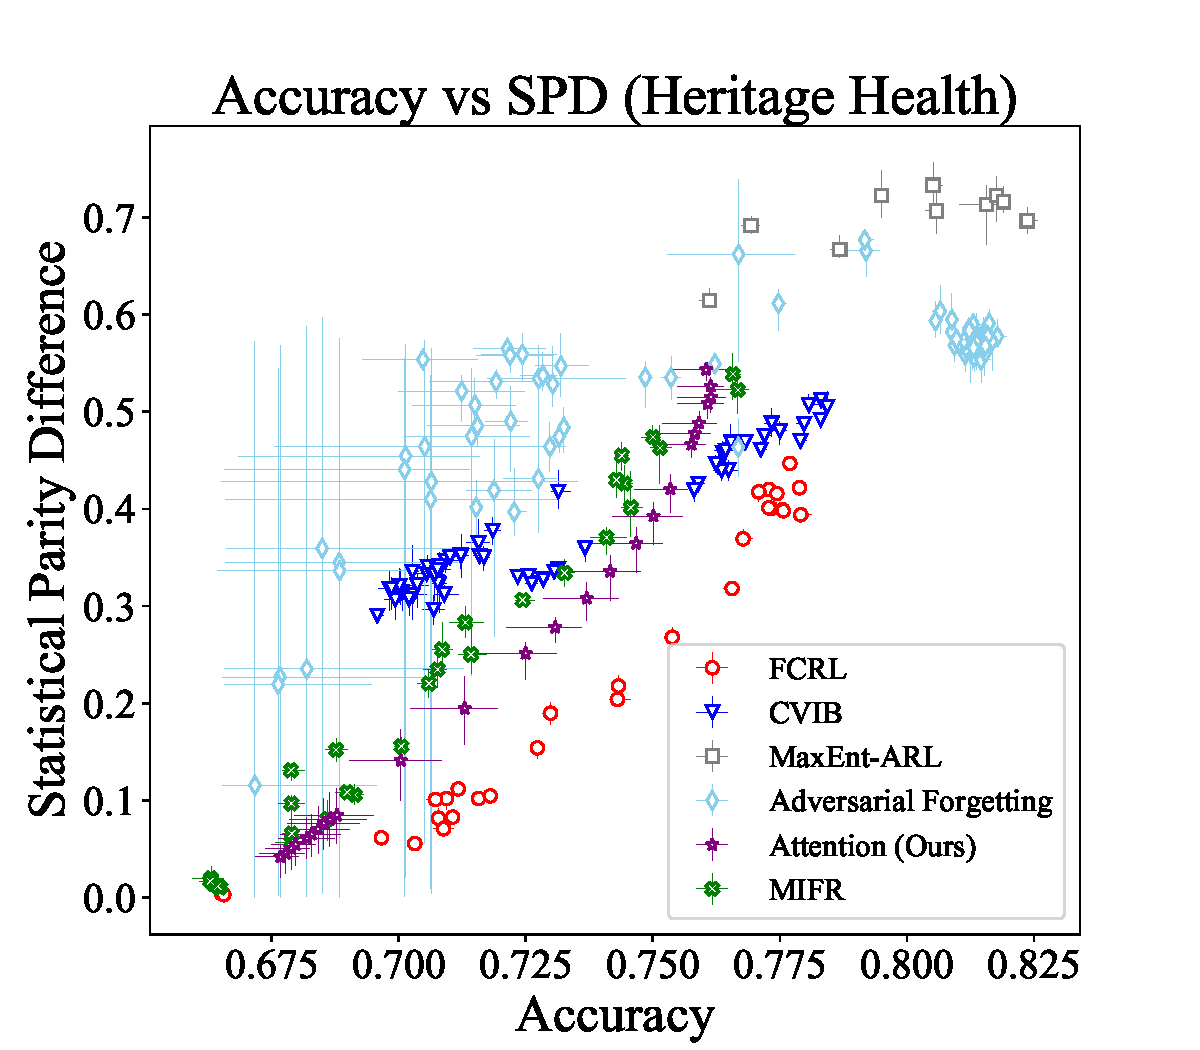
\includegraphics[width=\textwidth,trim=0cm 0cm 1.8cm 1cm,clip=true]{./images/mitig_imgs/health_results_err.pdf}
    \end{subfigure}
    \caption{Accuracy vs parity curves for UCI Adult and Heritage Health datasets.}
    \label{fig:mitig_results}
\end{figure*}

As we have highlighted earlier, understanding how the information within features interact and contribute to the decision making can be used to design effective bias mitigation strategies. One such example was shown in Sec. ~\ref{sec:interpret_fairness}. Often real-world datasets have features which cause indirect discrimination, due to which fairness can not be achieved by simply eliminating the sensitive feature from the decision process. 
Using the attributions derived from our attention-based interpretability framework, we propose a post-processing mitigation strategy. Our strategy is to intervene on  attention weights as discussed in Sec.~\ref{mitig_sec}. We first attribute and identify the features responsible for the unfairness of the outcomes, i.e., all the features whose exclusion will decrease the bias compared to the original model's outcomes and gradually decrease their attention weights to zero. We show that this procedure provides competitive trade-offs compared to several recently fair machine learning approaches. 

\subsubsection{Experiments with Tabular Datasets}
\paragraph{Datasets, Baselines, and Evaluation Procedure:}
Most of the fair decision-making algorithms are benchmarked on tabular datasets. To this end, we evaluate our approach on two real-world datasets, \textit{UCI Adult} and \textit{Heritage Health}. In this section, we use statistical parity as our notion of fairness. However, due to the flexibility of our interpretability framework, it can  easily be extended to other fairness measures (discussed in Appendix Section A).  We compare our method against several recent baselines that are specifically optimized to achieve statistical parity. %We select two broad classes of methods as our baselines. %information-theortic, and adversarial. %In particular,  we compare with information-theoretic methods like \textit{\textbf{FCRL}}, \textit{\textbf{MIFR}} and \textit{\textbf{CVIB}}.  
Specifically,  we consider methods that use information-theoretic objectives to learn representations of data so that information about sensitive attributes is eliminated.
\textit{\textbf{CVIB}}~\cite{NEURIPS2018_415185ea} realize this objective through a conditional variational autoencoder, whereas \textit{\textbf{MIFR}}~\cite{pmlr-v89-song19a} used a combination of information bottleneck term and adversarial learning to optimize the fairness objective. 
\textit{\textbf{FCRL}}~\cite{gupta2021controllable} showed that optimizing information theoretic objectives can be used to achieve good trade-offs between fairness and accuracy by using specialized contrastive information estimators~\cite{gupta2021controllable}. 
In addition to information-theoretic approaches, we also considered baselines that use adversarial learning such as \textit{\textbf{MaxEnt-ARL}}~\cite{roy2019mitigating}, \textit{\textbf{LAFTR}}~\cite{pmlr-v80-madras18a}, and \textit{\textbf{Adversarial Forgetting}}~\cite{advforg}. 

For all these fair representation learning  baselines, we used the approach outlined in~\cite{gupta2021controllable} for training a downstream classifier and evaluating the accuracy/fairness trade-offs. The downstream classifier was a 1-hidden-layer MLP with 50 neurons along with ReLU activation function. Our experiments were performed on Nvidia GeForce RTX 2080. Each method was trained with five different seeds, and we report the average accuracy and fairness measure as statistical parity difference (SPD). \textit{\textbf{CVIB}}, \textit{\textbf{MaxEnt-ARL}}, \textit{\textbf{Adversarial Forgetting}} and \textit{\textbf{FCRL}} are designed for statistical parity notion of fairness and are not applicable for other measures like Equalized Odds and Equality of Opportunity.  \textit{\textbf{LAFTR}} can only deal with binary sensitive attributes and thus not applicable for Heritage Health dataset. For our approach, we vary the attention weights and report the resulting fairness-accuracy trade offs.  

Note that in contrast our approach,  the baselines described above are not interpretable as they  are incapable of directly attributing features to fairness outcomes.

% To measure the effectiveness of our interpretability framework and the inter of the attention weights as a bias mitigation strategy, we compared our mitigation results with different baselines. The results can also help us to notice that attention weights capture important information utilizing which in a smart manner can achieve us fairness. For our baselines, we included both  \textit{\textbf{MIFR}} also uses an information-theoretic objective to learn representations subject to fairness constraints~\cite{pmlr-v89-song19a}. 




% fairness, such as ~\cite{advforg} and \textit{\textbf{MaxEnt-ARL}}~\cite{roy2019mitigating}. We also utilized ~\cite{pmlr-v80-madras18a} on the Adult dataset as another baseline and reported its results; however, since this method is feasible for binary sensitive attributes only, we were unable to use it on the in which we have non-binary sensitive features.






% , we decided to perform our main experiments with this notion of fairness. In our later experiments on text data, we utilized another fairness notion to highlight this flexibility. Additional results on other fairness measures and baseline methods can be found in our supplementary material. 



% As discussed previously, it is important to know how features interact and contribute to the decision making outcome specifically if we want to design mitigation strategies. One obvious example was shown in Section \ref{syn_data_sec}: When there is the effect of the indirect discrimination, it is not enough to just blindly put the focus on the sensitive feature; however, knowing how features interact and contribute to the outcome can help in designing such mitigation strategies. In light of this, we propose a post-processing mitigation strategy that manipulates attention weights as discussed in Section \ref{mitig_sec}. We first use our interpretability framework to identify the features that are responsible for fairness of the model (all the features whose exclusion will decrease the bias compared to the original model) and gradually decrease their attention weights to zero. We used two real-world datasets and compared our mitigation technique with different mitigation strategies. We used statistical parity as our notion of fairness; however, due to the flexibility of our interpretability framework, our mitigation strategy can be extended to other fairness measures as well. Here, to compare our method against baselines that are mostly specifically optimized to achieve statistical parity, we decided to perform our main experiments with this notion of fairness. In our later experiments on text data, we utilized another fairness notion to highlight this flexibility. Additional results on other fairness measures and baseline methods can be found in our supplementary material. Each method was ran over five different seeds, and we reported the average of the accuracy and statistical parity difference (SPD). The downstream classifier was a 1-hidden-layer MLP with 50 neurons along with ReLU activation function. Our experiments were performed on Nvidia GeForce RTX 2080.
% \begin{figure*}[t]
% \begin{subfigure}[b]{0.49\textwidth}
% 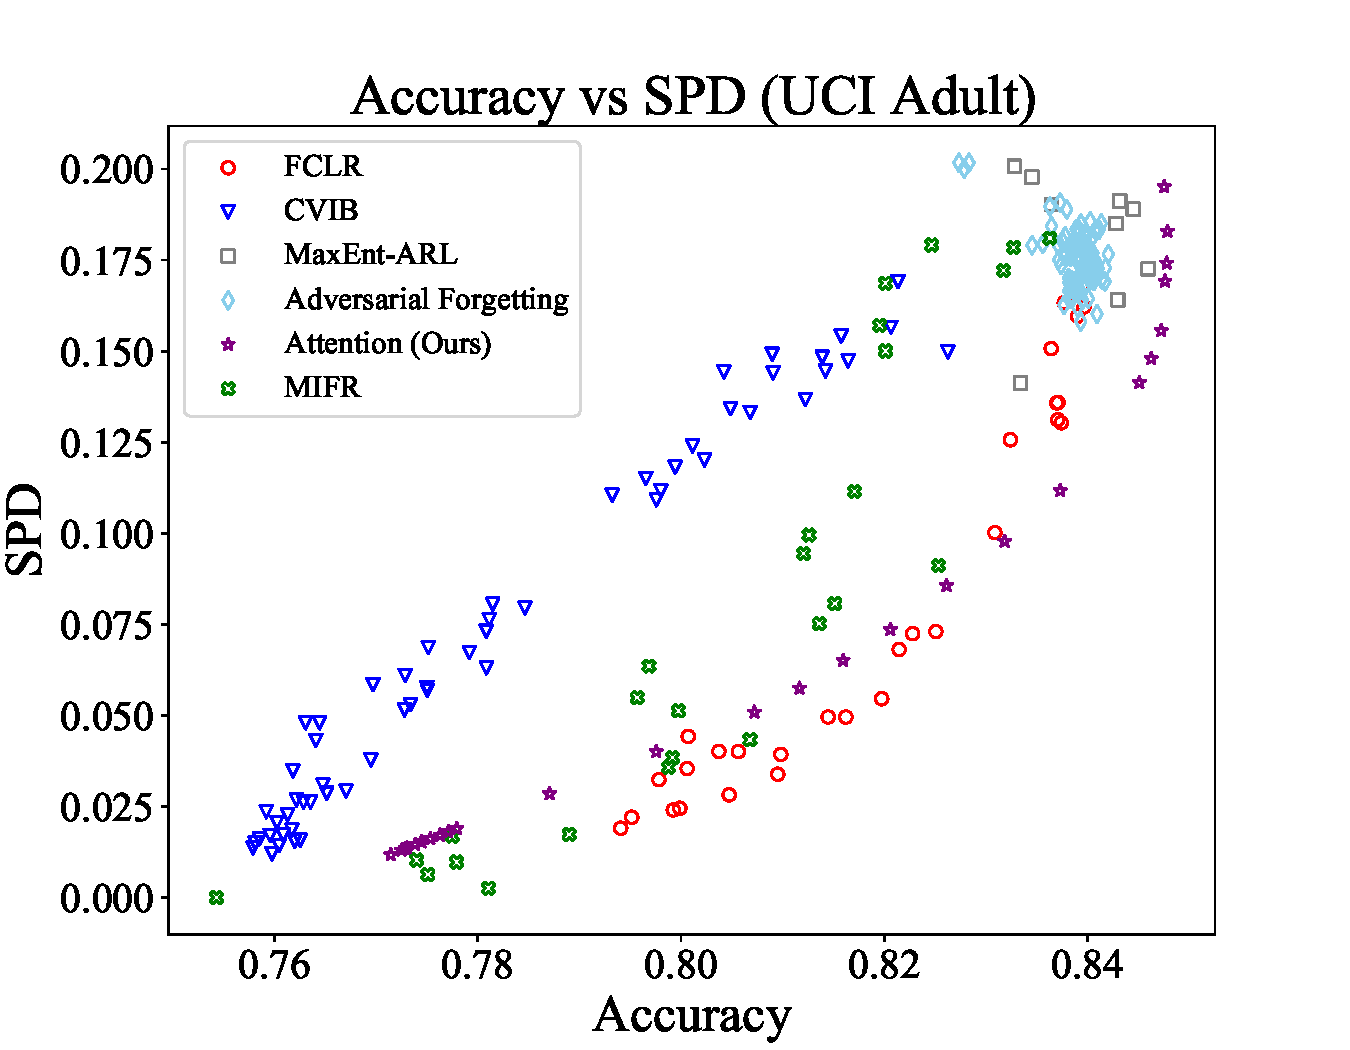
\includegraphics[width=\textwidth,trim=0cm 0cm 1.8cm 1.0cm,clip=true]{./images/mitig_imgs/adult_results.pdf}
% \end{subfigure}
% \begin{subfigure}[b]{0.49\textwidth}
% 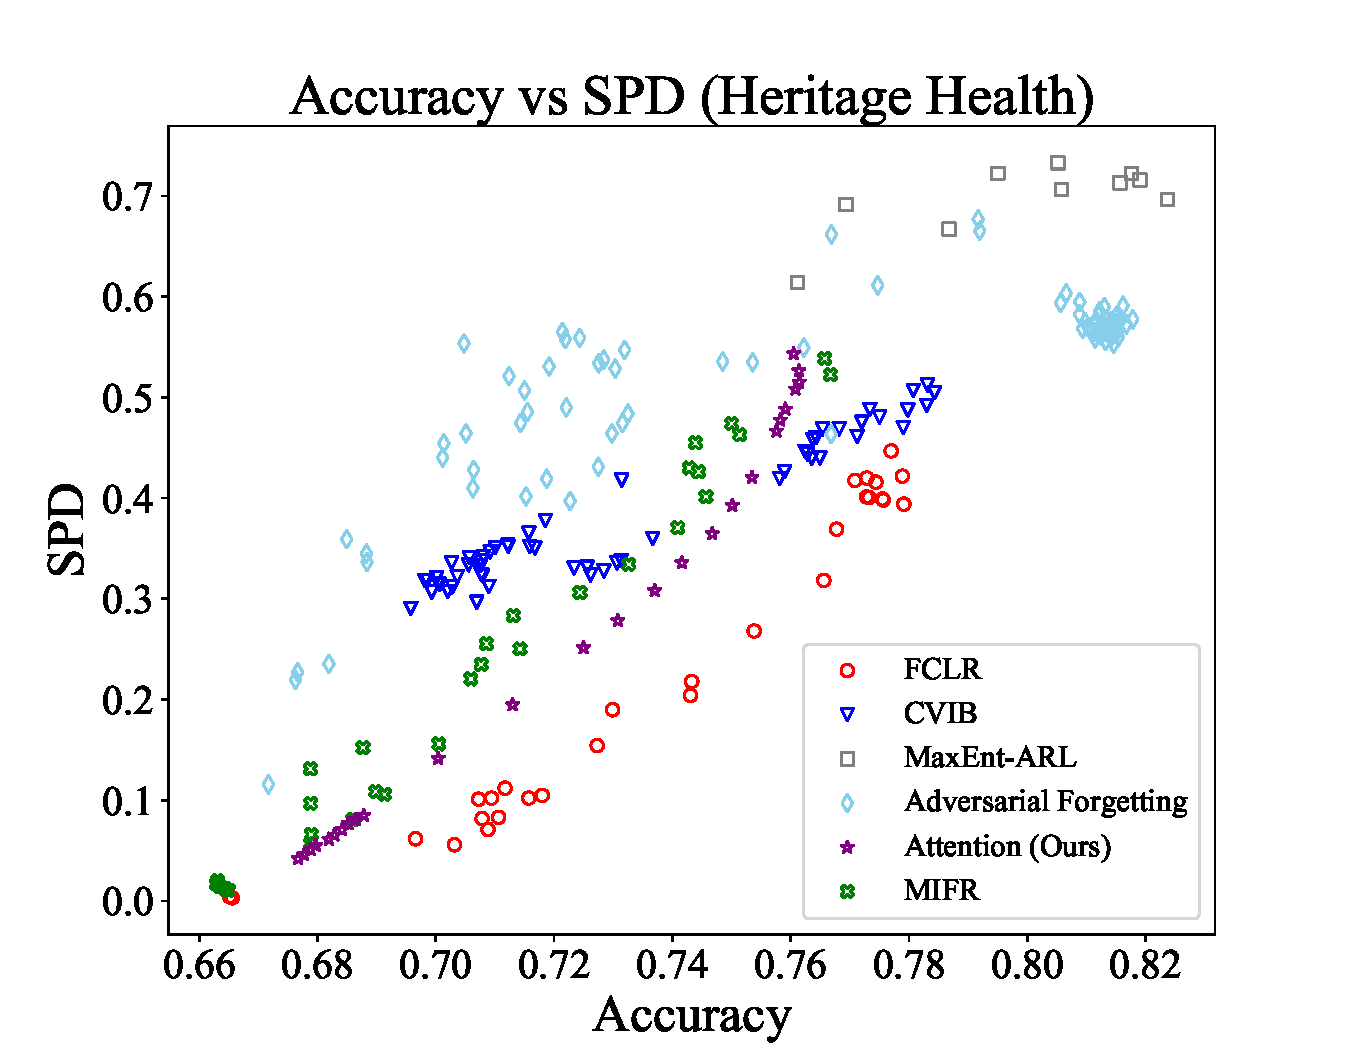
\includegraphics[width=\textwidth,trim=0cm 0cm 1.8cm 1cm,clip=true]{./images/mitig_imgs/health_results.pdf}
% \end{subfigure}
% \caption{Accuracy vs parity curves for UCI Adult and Heritage Health datasets.}
% \label{mitig_results}
% \end{figure*}


% \subsubsection{Data}
% We conduct our experiments on two real-world datasets-- UCI Adult~\cite{Dua:2019} and Heritage Health \footnote{https://www.kaggle.com/c/hhp} datasets. The UCI Adult dataset contains information about individuals with the prediction task of whether the income of the individual is greater than \$50k or not. The Heritage Health dataset contains patient information and the task is to predict the Charleson Index (comorbidity index which is a patient survival indicator). We used the same pre-processing and train-test splits as in~\cite{gupta2021controllable}. For the UCI Adult dataset we considered gender as the sensitive attribute and age as the sensitive attribute for the Herigate Health dataset.

% \paragraph{Baselines}
% To measure the effectiveness of our interpretability framework and the manipulation of the attention weights as a bias mitigation strategy, we compared our mitigation results with different baselines. The results can also help us to notice that attention weights capture important information utilizing which in a smart manner can achieve us fairness. For our baselines, we included both information-theoretic as well as adversarial approaches that try to achieve  fairness. \textit{\textbf{FCLR}} is a recent approach that learns representations to control parity through mutual information based on contrastive information estimators~\cite{gupta2021controllable}. \textit{\textbf{CVIB}} also tries to learn fair representations through an information-theoretic approach that optimizes an objective which would minimize the mutual information between the encoding and the sensitive attribute without adversarial training~\cite{NEURIPS2018_415185ea}. \textit{\textbf{MIFR}} also uses an information-theoretic objective to learn representations subject to fairness constraints~\cite{pmlr-v89-song19a}. In addition to information theoretic approaches, we also compared our results with adversarial approaches that try to achieve invariance and fairness, such as \textit{\textbf{Adversarial Forgetting}}~\cite{advforg} and \textit{\textbf{MaxEnt-ARL}}~\cite{roy2019mitigating}. We also utilized \textit{\textbf{LAFTR}}~\cite{pmlr-v80-madras18a} on the Adult dataset as another baseline and reported its results; however, since this method is feasible for binary sensitive attributes only, we were unable to use it on the Heritage Health dataset in which we have non-binary sensitive features.

\paragraph{Results:}
Fig.~\ref{fig:mitig_results} compares fairness-accuracy trade-offs of different bias mitigation approaches. We desire outcomes to be fairer, i.e., lower values of \texttt{SPD} and to be more accurate, i.e., towards the right. 
Our mitigation framework based on the manipulation of the attention weights is competitive with state-of-the-art mitigation strategies. However, most of these approaches are  specifically designed and optimized to achieve parity and do not provide any interpretability. 
Our model can not only achieve comparable and competitive results, but it is also able to provide explanation such that the users exactly know what feature and by how much it was manipulated to get the corresponding outcome. Another advantage of our model is that it needs only one round of training. The adjustments to attention weights are made post-training, and thus it is possible to achieve different trade-offs. Moreover, our approach does not need to know sensitive attributes while training; thus, it could work with other sensitive attributes not known beforehand or during the training.  Lastly, here we merely focused on mitigating bias (as our goal was to show that the interpretability framework can identify problematic features and their removal would result in bias mitigation) and did not focus too much on improving accuracy and achieving the best trade-off curve. We manipulated attention weights of all the features that contributed to unfairness irrespective of if they helped maintaining high accuracy or not. However, the trade-off results can be improved by carefully considering the trade-off each feature contributes to with regards to both accuracy and fairness (e.g., using results from Fig.~\ref{fig:interpret_results}) to achieve even  better trade-off results which can be investigated as a future direction (e.g., removing problematic features that contribute to unfairness only if their contribution to accuracy is below a certain threshold value). Picking the right threshold value is challenging and needs further investigation.



% light on the importance of the interpretability framework and that it correctly captures how features interact and contribute to fairness of the system as knowing these types of information one can design strategies that can benefit the outcome. The results show the averaged accuracy vs parity curves for five different runs over various random seeds. Having results in the bottom-right corner is the ideal case as it represents the region with the highest accuracy and lowest bias. 



% \subsubsection{Results}
% From the results demonstrated in Fig.~\ref{fig:mitig_results}, one can observe that our mitigation framework based on the manipulation of the attention weights is comparable to state of the art mitigation strategies that are specifically targeted and optimized to achieve parity without providing interpretable outcomes. This sheds light on the importance of the interpretability framework and that it correctly captures how features interact and contribute to fairness of the system as knowing these types of information one can design strategies that can benefit the outcome. The results show the averaged accuracy vs parity curves for five different runs over various random seeds. Having results in the bottom-right corner is the ideal case as it represents the region with the highest accuracy and lowest bias. Our model is not only able to achieve comparable and competitive results, but it is also able to provide explanation such that we exactly know what feature and by how much it was manipulated to get the corresponding outcome. It addition, our approach needs only one round of training to get all the trade-off results for every possible sensitive attribute that might exist. Lastly, here we merely focused on mitigating bias (as our goal was to show that the interpretability framework is able to identify problematic features; thus, their removal would result in bias mitigation) and did not focus too much on improving accuracy and achieving the best trade-off curve. Therefore, we manipulated attention weights of all the features which contributed to unfairness irrespective of if they helped maintaining high accuracy or not. However, the trade-off results can be improved by considering the trade-off each feature contributes to with regards to both accuracy and fairness (e.g. using results from Fig.~\ref{fig:interpret_results}) for a stronger trade-off results which can be investigated as a future direction (e.g. removing problematic features that contribute to unfairness only if their contribution to accuracy is below a certain threshold value). Picking the right threshold value can be a challenge on its own that would need further investigation.
\vspace{-0.3cm}
\subsubsection{Experiments with Non-Tabular Data}
\vspace{-0.1cm}
\begin{table}[t]
\centering
\begin{tabular}{ p{3.5cm} c c c}
 \toprule
\textbf{Method}&\textbf{Dentist TPRD (stdev)}&\textbf{Nurse TPRD (stdev)}&\textbf{Accuracy (stdev)}\\
 \midrule
 \parbox[t]{2mm}{\multirow{1}{*}{\shortstack[l]{Post-Processing (Ours)}}}
&\textbf{0.0202 (0.010)}&\textbf{0.0251 (0.020)}&0.951 (0.013)\\[0.5pt]

 \parbox[t]{2mm}{\multirow{1}{*}{\shortstack[l]{Pre-Processing}}}
&0.0380 (0.016)&0.0616 (0.025)&0.946 (0.011)\\[0.5pt]
\midrule
 \parbox[t]{2mm}{\multirow{1}{*}{\shortstack[l]{Not Debiased Model}}}
&0.0474 (0.025)&0.1905 (0.059)&\textbf{0.958 (0.011)}\\[0.5pt]

%  \midrule

%  \midrule
 \bottomrule
\end{tabular}
 \caption{Difference of the True Positive Rates (TPRD) amongst different genders for the dentist and nurse occupations on the biosbias dataset. Our introduced post-processing method is shown to be the most effective in reducing the disparity for both occupations compared to the previously used pre-processing technique.}
\label{bios_results}
\end{table}
\begin{figure}[t]
    \centering
    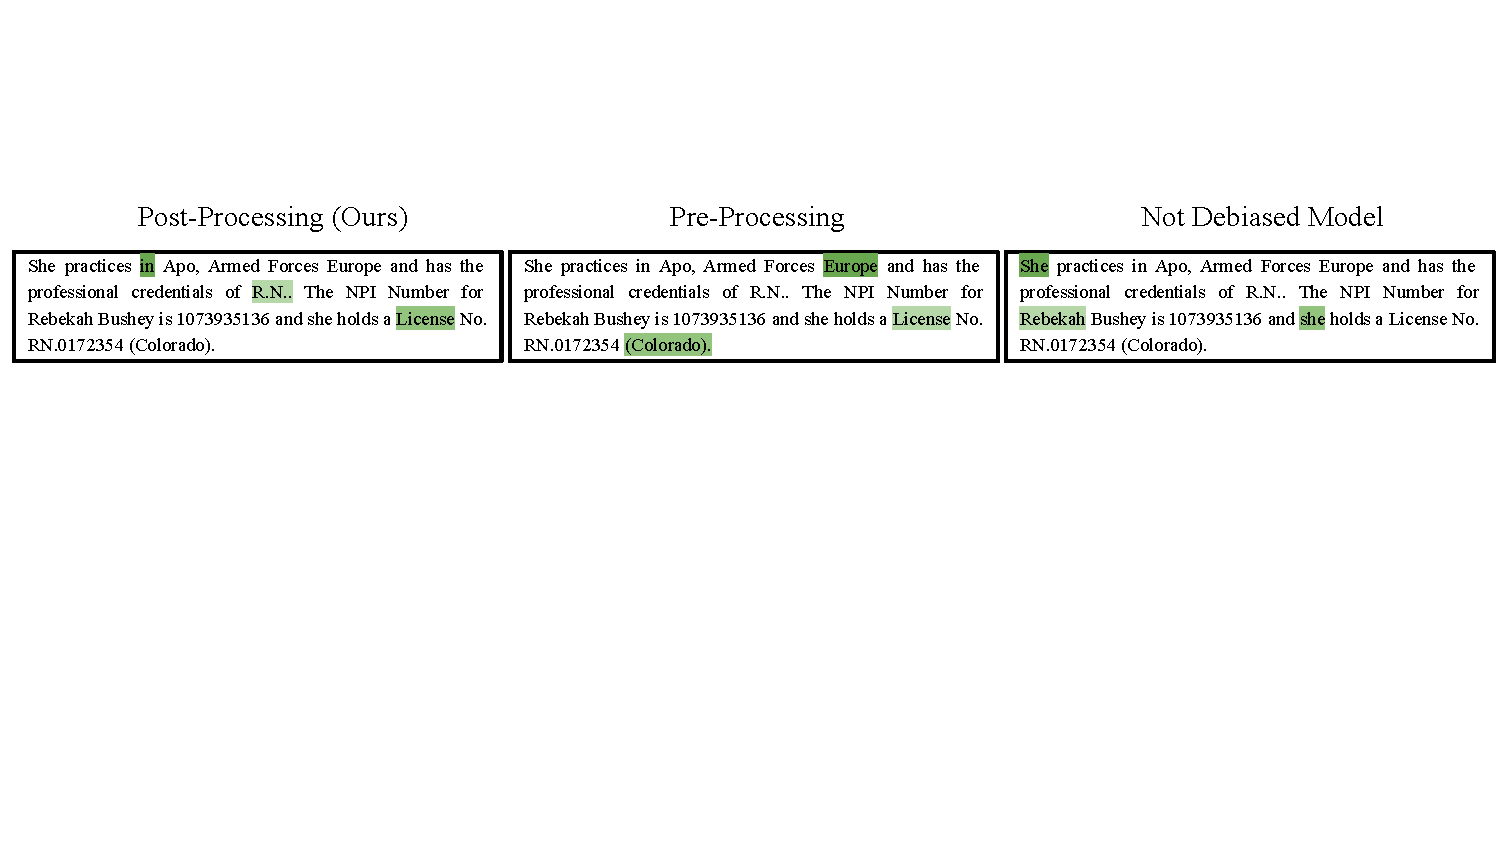
\includegraphics[width=\textwidth,trim=0cm 8cm 0cm 3cm,clip=true]{./images/NLP_qual/ex1.pdf}
     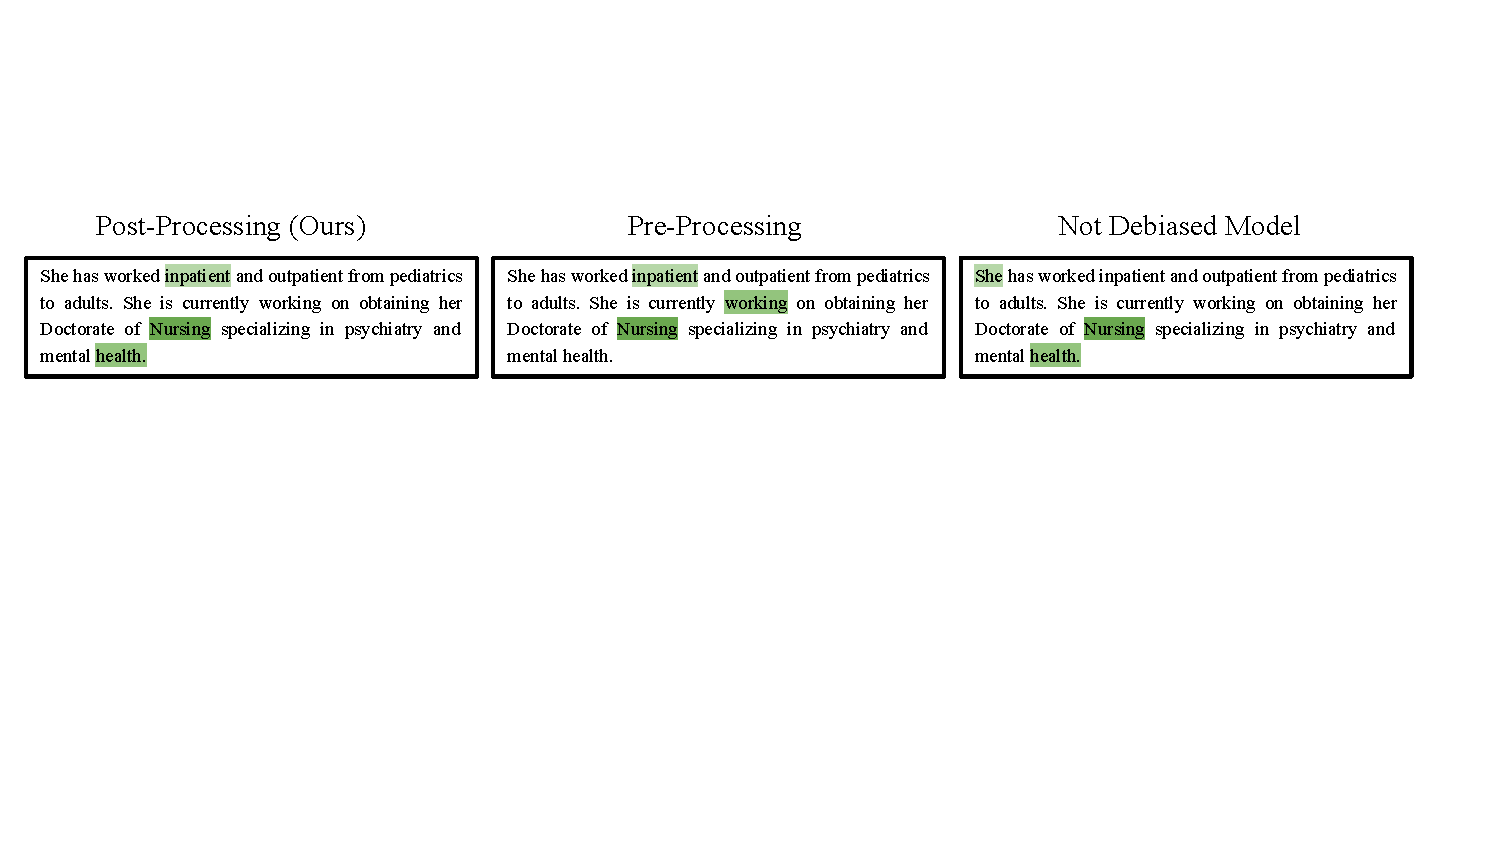
\includegraphics[width=\textwidth,trim=0.24cm 7cm 1.4cm 3cm,clip=true]{./images/NLP_qual/ex2.pdf}
    \caption{Qualitative results from the non-tabular data experiment on the job classification task based on the bio texts. Green regions represent top three words that the model used for its prediction based on the attention weights. While the Not Debiased Model mostly focused on gendered words, our method focused on more useful words, such as R.N. (Registered Nurse), to predict the nurse label for the corresponding bio.}
    \label{NLP_qualitative}
\end{figure}

In addition to providing interpretability, our approach is flexible and useful for controlling fairness in modalities other than tabular datasets. To put this to the test, we applied our model to mitigate bias in text-based data. We consider the \textit{biosbias} dataset~\cite{de2019bias}, and  use our mitigation technique to reduce observed biases in the classification task performed on this dataset. We compare our approach with the debiasing technique proposed in the original paper~\cite{de2019bias}, which works  by masking the gender-related words and then training the model on this masked data. As discussed earlier, such a method is computationally inefficient. It requires  re-training the model or creating a new masked dataset, each time it is  required to debias the model against different attributes, such as gender vs. race. 
For the baseline pre-processing method, we masked the gender-related words, such as names and gender words, as provided in the biosbias dataset and trained the model on the filtered dataset. On the other hand, we trained the model on the raw bios for our post-processing method and only manipulated attention weights of the gender words during the testing process. Notice, we eliminated the same features for both of the methods. Only the time of the elimination was different (one before training and one after training by manipulating the attention weights).


In order to measure the bias, we used the same measure as in~\cite{de2019bias} which is based on the equality of opportunity notion of fairness~\cite{NIPS2016_9d268236} and reported the True Positive Rate Difference (TPRD) of each occupation amongst different genders. As shown in Table~\ref{bios_results}, our post-processing mitigation technique provides lower TRPD while being more accurate, followed by the technique that masks out the gendered words before training. Although both methods reduce the bias compared to a model trained on raw bios without applying any mask or invariance to gendered words, the post-processing method is more effective. 
Fig.~\ref{NLP_qualitative} also shows some qualitative results and highlights the differences between models in terms of their most attentive features for the prediction task. As shown in the results, our post-processing technique is able to use more meaningful words, such as R.N. which stands for registered nurse, to predict the outcome label nurse, while the not debiased model focuses on gendered words.


% The second approach, however, is our proposed mitigation technique based on post-processing that trains the model on the original corpus without masking, but masks out (zeros out the attention weights) the effect of undesired features during test time. This method is more efficient since it does not require retraining for debiasing with regards to different attributes as debiasing happens during test time.




% In addition to providing interpretability, an advantage of our proposed model over non-neural based models is its flexibility to be applied to large scale datasets as well as large text-based data. To put this into test, we applied our model over a text-based data and used our mitigation technique based on attention weight manipulation to reduce observed biases in the classification task performed on the dataset. The results confirm the effectiveness of our framework.
% \subsubsection{Data}
% \subsubsection{Results}

% For our results, we considered two approaches for bias mitigation. The first approach, is what is used in some previous work~\cite{de2019bias} to debias the results. This method is based on pre-processing and works by masking the gender words and training the model. As explained previously, these types of pre-processing methods are not efficient since they require re-training the model each time we require to debias the model against different attributes, such as gender vs race. The second approach, however, is our proposed mitigation technique based on post-processing that trains the model on the original corpus without masking, but masks out (zeros out the attention weights) the effect of undesired features during test time. This method is more efficient since it does not require retraining for debiasing with regards to different attributes as debiasing happens during test time.

% For the baseline pre-processing method, we masked out the gender related words, such as names and gender words, as also provided in the biosbias dataset and trained the model on the filtered dataset. On the other hand, for our post-processing method, we trained the model on the raw bios and only manipulated attention weights of the gender words during the testing process. Notice, we eliminated the same features for both of the methods. Only the time of the elimination was different (one before training and one after training by manipulating the attention weights).

% In order to measure the bias, we used the same measure as in ~\cite{de2019bias} which is based on the equality of opportunity notion of fairness~\cite{NIPS2016_9d268236} that reports the True Positive Rate Difference (TPRD) of each occupation amongst different genders. As shown in Table~\ref{bios_results}, our introduced post-processing mitigation technique that works by manipulating the attention weights, works the best in minimizing the bias for both occupations followed by the in-processing technique that masks out the gendered words before training. Although both methods reduce the bias compared to a model that is trained on raw bios without applying any mask or invariance to gendered words, the post-processing method achieves the best results. It also has the advantage of not needing retraining for debiasing with regards to different aspects aside from gender such as race. Fig.~\ref{NLP_qualitative} also shows some qualitative results and highlights the differences between models in terms of their most attentive features for the prediction task. As shown in the results, our post-processing technique is able to use more meaningful words, such as R.N. which stands for registered nurse, to predict the outcome label nurse, while the not debiased model focuses on gendered words.



